\begin{abstract}
User-set-rate stablecoins defend their dollar peg through a continuous reverse priority queue in which borrowers post interest rates to avoid par redemptions. Using 44,907 Ethereum events across 485~days (964 troves, 23 managers, 37 on-chain permission tuples) for Liquity V2's BOLD, we uncover a cost inversion in borrower-side delegation. Delegated loans quote 40.15~bp lower base APR in Development (408~days) and 55.44~bp lower in Confirmation (77~days), yet incur 38.04~BOLD per million debt-days higher liability (5.76\% versus 3.97\% pooled financial cost) because 7-day repricing penalties total 421,986.60~BOLD, 93.73\% from premature hikes. Separating 604,800-second revert walls reveals sharp 168-hour cut bunching ($b = 91.8$, $p = 1.57 \times 10^{-34}$), a 57.8~percentage-point hike-versus-cut asymmetry, and live spike-and-cut arbitrage extracting 84.02\% and 60.96\% discounts. Bartik shift-share 2SLS on mechanical routing swings identifies causal 48-hour fee surges ($+13.53$~BOLD/M debt-days), while multivariate Hawkes models isolate cross-manager leapfrogging ($\hat{\alpha}_{\text{cross}} \in [0.17, 0.65]$). Within-day GPV inversion recovers a 362.0~bp median disruption cost; symmetric incremental fees (4.06\%) and one-slot rate-bond escrow (3.85\%) eliminate spike-and-cut arbitrage and place delegated BOLD below Aave GHO (4.54\%), Aave USDC (5.30\%), Curve crvUSD (5.68\%), and Sky (7.88\%--8.88\%).
\end{abstract}

\vspace{0.35em}
\noindent\textit{JEL Classification:} G23, G12, G14, D47, D82.

\noindent\textit{Keywords:} Stablecoins, delegated rate management, priority queues, cooldown notch bunching, nonparametric auction inversion, decentralized finance.

\vspace{0.6em}

\section{Introduction}\label{sec:intro}

Decentralized stablecoins confront a classic monetary commitment dilemma: how to hold a one-dollar peg without vesting discretionary policy power in a centralized issuer \citep{davernas2026can,ma2026stablecoin,goel2026making}. Liquity V2 addresses this problem through an immutable market mechanism for its BOLD stablecoin. Borrowers against Ethereum collateral (WETH, wstETH, and rETH) choose their own annual interest rates, and the protocol defends the dollar peg by routing par redemptions in ascending order of posted rates \citep{liquity2024whitepaper,liquity2024docs}. Borrowers who quote higher rates move to the back of a reverse priority queue and avoid redemption disruption. Because active queue management demands continuous attention, third-party delegated batch managers rapidly captured the market, expanding from 8.59\% of canonical BOLD debt on June 30, 2025 to 59.06\% by June 30, 2026, with the top three manager addresses controlling 86.04\% of managed debt-day exposure across our Development book. The same codebase has scaled across nine licensed deployments on Ethereum, Hyperliquid, Arbitrum, Flare, Scroll, and Swellchain, reaching a simultaneous peak total value locked (TVL) of \usd425.06~million on July 14, 2025 (\usd524.57~million summing individual peaks).

Quoted interest rates conceal the true price of delegation. Across our 408-day Development sample (May 19, 2025 through June 30, 2026; 72,070 loan-days), delegated loans quote a debt-weighted base APR 40.15~bp below self-managed loans conditional on branch-by-day fixed effects and loan covariates (95\% 14-day circular block-bootstrap CI $[-53.06, -28.23]$~bp). In our frozen 77-day chronological Confirmation holdout (July 1 through September 15, 2026; 13,607 loan-days), that quoted base discount widens to 55.44~bp ($[-77.49, -31.35]$~bp), and all-in quoted APR (base plus management fee) remains 12.62~bp lower in Development ($[-25.29, -1.28]$~bp) and 27.20~bp lower in Confirmation ($[-48.63, -2.55]$~bp). Exact liability accounting reverses that ranking completely. Delegated debt accrues 153.04~BOLD per million debt-days in Development versus 115.00~BOLD for self-managed debt, an excess cost of $+38.04$~BOLD per million debt-days (95\% CI $[+10.86, +67.34]$), or 5.76\% versus 3.97\% in annualized pooled financial borrowing cost across all 485~days. The culprit is Liquity V2's cooldown fee. Any rate adjustment within 168~hours (7~days) of a prior change assesses an upfront fee equal to seven days of the branch's entire average borrowing rate multiplied by total batch debt, capitalized directly onto borrower principal. Over 485~days, batch managers triggered 421,986.60~BOLD in repricing penalties, 93.73\% (395,542.67~BOLD) from 308 consecutive premature upward adjustments, turning delegated BOLD from cheaper than Aave V3 GHO (4.54\%), Aave V3 USDC (5.30\%), and Curve crvUSD (5.68\%) into more expensive.

Contractual incidence separates control from payment. Unlike supply-side vault curators in modular lending protocols such as Morpho and Euler, who manage lender assets to maximize depositor yield \citep{chitra2025curationary,zbandut2025institutionalizing,mancino2026sok}, Liquity V2 batch managers run liability-side delegation inside a competitive avoidance queue. Managers earn a percentage fee on debt principal. They pay negligible Ethereum gas to adjust rates, face reputational outflows after visible redemptions, and leave borrowers absorbing 100\% of every capitalized cooldown penalty. Worse still, because the smart contract adds each upfront penalty directly into \texttt{newDebt} before computing future management fees, premature churning mechanically expands a manager's own revenue base. Small rate steps thus inflict steep borrower losses.

This paper brings five empirical and structural findings to bear on delegated interest-rate management, cooldown friction, and stablecoin welfare using the complete 485-day canonical Ethereum mainnet ledger (44,907 events across 11,444 transactions, 964 unique troves, and 23 unique manager addresses) augmented with live RPC contract state and cross-protocol market prices. First, permission metadata separates legal constraints from economic choices. Recovering all 37 immutable on-chain manager permission tuples at block 26,478,046 reveals that 12 manager-branch registrations hardcode a 604,800-second minimum change period, generating a smart-contract revert wall that accounts for 81.0\% (260 of 321) of the raw zero-debt spike at 168~hours while incurring 0.00~BOLD in fees across 395 genuine updates. Restricting to managers who face the economic fee notch (minimum change periods of 1~hour or 24~hours, where 1-hour-floor managers generate 95.3\% of all 421,986.60~BOLD in borrower penalties) isolates clean optimization at the 168-hour boundary. Positive-debt delegated cuts show sharp bunching. Across 90 cuts, zero occur in $[120\text{h}, 168\text{h})$ while 22.2\% arrive in the first free hour $[168\text{h}, 169\text{h})$ (normalized bunching $b = 91.8$, 95\% CI $[45.4, 153.7]$, binomial $p = 1.57 \times 10^{-34}$). Positive-debt delegated hikes break the cooldown 65.6\% of the time (345 of 526), 57.8~percentage points above delegated cuts ($p = 2.00 \times 10^{-26}$) and 36.3~percentage points above self-managed individual hikes (29.3\%, $p = 2.92 \times 10^{-36}$). Inside the final four hours $[164\text{h}, 168\text{h})$, managers executed eight paid premature hikes totaling 11,979.39~BOLD despite zero binding rate caps, four of which (10,567.89~BOLD) occurred with zero branch redemptions in the preceding and subsequent six hours, including an M05 wstETH hike 3.2~minutes before free expiry costing 1,331.98~BOLD and an M01 wstETH hike 220.4~minutes early costing 9,207.19~BOLD.

Second, two live mainnet exploits expose downward fee underpricing. Forensic inspection of all 1,712 batch updates documents two simultaneous spike-and-cut arbitrage episodes on March 6, 2026 (15:50:47 to 16:51:23~UTC, elapsed time 1.01~hours) that exploit the fixed branch-average cut fee. On wstETH (7.98~million~BOLD debt), manager M01 spiked its rate freely from 0.70\% to 10.50\% and cut back to 0.70\% one hour later, paying 2,307.13~BOLD in cut fees plus 90.19~BOLD in excess interest versus 15,001.39~BOLD for an honest 7-day hold, an 84.02\% total-excess discount (84.62\% comparing cut fee to 7-day excess interest). Simultaneously on WETH (1.79~million~BOLD debt), M03 spiked from 3.10\% to 13.10\% and reversed to 3.30\% at a 60.96\% total-excess discount (61.56\% cut fee versus 7-day hold). Both episodes break Liquity V2's Status Quo rule as well as a naive increment-only hike patch (baseline $\DesignA$), which leaves downward cut fees capped at the branch average and renders a third Confirmation episode profitable. Replaying exact contract state across all 485~days shows that the zero-storage symmetric incremental rule ($\DesignAStar$) reduces borrower repricing fees by 83.8\% ($-353{,}559.31$~BOLD) and hardened one-slot principal-escrow ($\DesignD$) reduces all-in costs by 93.5\% ($-394{,}659.70$~BOLD including 5\% lockup opportunity cost, with zero escrow underflows), while driving positive spike-and-cut arbitrage gains on every episode to 0.000\%. We also scan all 481 batch join, removal, and switch operations, finding 17 rate-lowering transitions within seven days of a prior hike and zero profitable bypasses, establishing that patching all four rate-transition entry points closes a proactive zero-day loophole.

Third, mechanical redemption routing breaks voluntary-delegation selection bias. Inside Liquity V2's \texttt{CollateralRegistry}, every redemption transaction splits dollar volume across collateral branches strictly in proportion to each branch's unbacked debt (total debt minus Stability Pool deposits). Reconstructing 1,708 multi-branch redemption transactions out of 1,709 exposes 100-fold routing swings, including a spring 2026 collapse of WETH routing share from 70.4\% to 0.0\% while wstETH rose to 97.5\%. In loan-day panel regressions with Trove and Branch-by-Day fixed effects, delegated loans raise base rates differentially with predetermined trailing 7-day average routing share ($+73.06$~bp pooled, $p = 0.0378$; $+110.04$~bp Development, $p = 0.0004$). Predetermined Bartik shift-share 2SLS regressions \citep{borusyak2022quasi} yield strong first stages ($F = 197.7$ pooled) and identify a causal 48-hour upfront fee surge of $+13.53$~BOLD per million debt-days ($p = 0.0347$ with exact fixed-effect degrees-of-freedom adjustment; Driscoll--Kraay $L=2$ $p = 0.0810$; 14-day circular block-bootstrap 95\% CI $[+2.78, +35.02]$), corroborated by null future placebo leads ($t+7\text{d}$: $+3.58$, $p = 0.664$) and manager-panel 2SLS ($+29.71$~BOLD per million debt-days across all 21 positive-debt managers, $F = 241.1$). Rival escalation amplifies these shocks. Estimating multivariate Hawkes point-process models \citep{hawkes1971spectra,ogata1988statistical} with exact analytical time-rescaling integrals and free exogenous redemption-decay half-lives (down to 0.49~minutes) isolates cross-manager leapfrogging across all six positive-debt branch-samples ($\hat{\alpha}_{\text{cross}} \in [0.17, 0.65]$, likelihood-ratio statistics 13.1 to 312.2, $p \le 2.89 \times 10^{-4}$), attributing 21.77\% (89,543.95~BOLD) of pooled hike penalties to cross-manager contagion.

Fourth, gas savings cannot explain delegated borrowing costs. Matching 100.00\% of user and manager transactions (11,421 of 11,421; \usd31,566.77 total gas) shows that delegated gas economies ($-1.074$~BOLD per million debt-days) are 35~times too small to offset the repricing penalty. We then structurally invert the reverse priority queue following \citet{guerre2000optimal}. Matching 5,005 of 5,026 on-chain redemption hits onto pre-redemption queue ranks and inverting the debt-weighted average within-(branch, day) cross-sectional quantile curve eliminates a 3.18-fold macro-drift bias present in naive time pooling, recovering a 3.87\% absorber share and a realistic 362.0~bp median gross disruption cost (IQR $[94.6, 1{,}983.5]$~bp, in-sample quantile RMSE 2.8~bp). Solving the general-equilibrium Stability Pool yield feedback across supply elasticities $\varepsilon_{\text{SP}} \in \{0.00, 0.25, 0.50, 1.00, 2.00\}$ cleanly separates avoided pecuniary transfers to Stability Pool and liquidity-incentive recipients from pure social deadweight loss. Both fee reforms reverse BOLD's market ranking. At baseline elasticity $\varepsilon_{\text{SP}} = 0.50$, $\DesignAStar$ cuts borrower observed financial cost by 170.5~bp (5.76\% to 4.06\%) and $\DesignD$ cuts it by 191.5~bp (to 3.85\%) while Stability Pool APR adjusts moderately from 4.97\% to 4.40\% and 4.34\%. Across our 485-day cross-protocol benchmark, these two reforms move delegated BOLD below Aave GHO (4.54\%), Aave USDC (5.30\%), Curve crvUSD (5.68\%--6.36\%), and Sky (7.88\%--8.88\%), while maintaining a 22.93~bp secondary-market peg RMSE that is 2.6~times tighter than Liquity V1 LUSD (59.33~bp).

This paper connects four strands of financial economics and market design. First, it extends the stablecoin stability literature \citep{davernas2026can,ma2026stablecoin,goel2026making,aldasoro2026stablecoin,klagesmundt2022while,lyons2023what,deblasis2023intelligent,ling2025sok} and empirical Liquity V1 evidence \citep{genc2026a,genc2026b} to user-set-rate peg defense, showing that manager concentration inside an immutable protocol creates a borrower-side parallel to the centralized arbitrage friction documented by \citet{ma2026stablecoin}. Second, it supplies the liability-side counterpart to classical delegated intermediation and churning models \citep{diamond1984financial,holmstrom1997financial,allen1993churning,admati1997does,scharfstein1990herd} and recent DeFi lending and vault curation studies \citep{gudgeon2020defi,schar2021defi,aramonte2021defi,cornelli2025why,chitra2025curationary,zbandut2025institutionalizing,mancino2026sok}. Third, it translates notch bunching \citep{kleven2013using}, blockchain priority-queue bidding \citep{afeche2004pricing,huberman2021monopoly}, and nonparametric auction inversion \citep{guerre2000optimal} to a continuous-time reverse priority queue. Formal proofs of equilibrium uniqueness, axiomatic characterization of $\DesignAStar$ and $\DesignD$, Lean~4 mechanization, and compiled EVM gas benchmarks appear in the companion theoretical paper \citep{companion2026}; this paper focuses on empirical identification, forensic mechanism replays, structural estimation, and cross-protocol welfare. Section~\ref{sec:setting} details the institutional mechanics, dataset, and testable predictions; Section~\ref{sec:notch} analyzes the 168-hour notch and agency friction; Section~\ref{sec:exploits} examines spike-and-cut exploits and fee-rule replays; Section~\ref{sec:causal} presents mechanical-routing causal identification and Hawkes leapfrogging; Section~\ref{sec:structural} develops gas accounting, within-day GPV estimation, equilibrium welfare, and the cross-protocol benchmark; Section~\ref{sec:conclusion} concludes.

\section{Institutional setting, data, and theoretical predictions}\label{sec:setting}

\subsection{Liquity V2 mechanics and contractual fee incidence}\label{subsec:mechanics}

Liquity V2 issues BOLD, a dollar-pegged overcollateralized stablecoin (1~BOLD targets \usd1 at par) backed by three isolated Ethereum collateral branches: WETH, wstETH, and rETH \citep{liquity2024whitepaper,liquity2024docs}. Each borrower opens a collateralized debt position (a trove) with minimum principal debt $\text{MIN\_DEBT} = 2{,}000$~BOLD and selects an annual interest rate $r_i \in [r_{\min}, r_{\max}] = [0.5\%, 250\%]$. Interest accrues continuously on trove principal and flows directly to protocol stakeholders without governance intermediation: 75\% ($\eta = 0.75$) pays Stability Pool (SP) depositors who provide BOLD liquidity to absorb liquidations, and 25\% ($1 - \eta = 0.25$) funds Protocol Incentivized Liquidity (PIL) for secondary-market DEX pools.

Peg defense relies on permissionless arbitrage redemptions. Whenever BOLD trades below \usd1 minus the protocol redemption fee $\phi$ on secondary markets, arbitrageurs can purchase BOLD and redeem it against the protocol for \usd1 worth of underlying collateral at oracle price, minus a dynamic redemption fee $\phi \ge \phi_{\min} = 0.5\%$ that rises with redemption volume and decays with a 6-hour half-life. Redeemed troves keep that fee. By contract design, \texttt{TroveManager} retains \texttt{collFee} inside the redeemed trove, retiring \usd1 of debt while removing \usd$(1 - \phi)$ of collateral. Across branches, \texttt{CollateralRegistry} splits every redemption transaction mechanically in proportion to each branch's unbacked debt, defined as total branch debt minus that branch's Stability Pool BOLD balance. Within each branch, redemptions execute in strict ascending order of posted annual interest rate $r_i$ (with LIFO tie-breaking among identical rates in \texttt{SortedTroves}). Low-rate troves absorb redemptions first; high-rate troves sit protected at the back.

To deter borrowers from quoting $r_{\min} = 0.5\%$ in quiet periods and jumping upward just before a redemption wave arrives, \texttt{BorrowerOperations} imposes a 7-day adjustment cooldown ($P = \text{UPFRONT\_INTEREST\_PERIOD} = 604{,}800$~seconds; year length $Y = 31{,}536{,}000$~seconds). Any rate change occurring at elapsed time $\Delta t < P$ since \texttt{lastInterestRateAdjTime} triggers an upfront fee equal to seven days of the projected branch-average interest rate $\bar{r}$ applied to the entire trove or batch debt $D$:
\begin{equation}\label{eq:sq_fee}
\Phi_{\SQ}(D, r_0, r_1, \bar{r}, \Delta t) =
\begin{cases}
D\,\bar{r}\,\dfrac{P}{Y}, & \text{if } \Delta t < P \text{ and } r_1 \ne r_0,\\[6pt]
0, & \text{if } \Delta t \ge P \text{ or } r_1 = r_0.
\end{cases}
\end{equation}
The same fee applies to initial debt origination, new debt draws, and joining a batch within cooldown, and all upfront fees route into the exact same 75\%/25\% SP/PIL split as recurring interest.

Borrowers may manage rates individually or delegate rate control to a registered batch manager \citep{liquity2024arm}. Upon registration in a collateral branch, a batch manager fixes three immutable on-chain parameters: a rate floor (\texttt{minInterestRate}), a rate ceiling (\texttt{maxInterestRate}), and a minimum change period (\texttt{minInterestRateChangePeriod}) bounded below by the protocol's 3,600-second (1-hour) limit, alongside an annual management fee capped at 10\% (empirically 0.00\%--0.30\%, median 0.30\%). All troves inside a batch share one clock. When a manager calls \texttt{setBatchManagerAnnualInterestRate} prematurely ($\Delta t < P$), two contract lines in \texttt{BorrowerOperations} create a stark principal-agent misalignment. First, the upfront fee capitalizes onto borrower principal (\texttt{newDebt += upfrontFee}). Borrowers bear 100\% of $\Phi_{\SQ}$ while the manager pays only gas $g_{\text{tx}}$. Second, future management fees accrue on the inflated debt balance (setting weighted management debt equal to \texttt{newDebt} times \texttt{annualManagementFee}), meaning premature updates mechanically expand the manager's annual fee stream by $+m_j \Phi_{\SQ}$.

\subsection{Canonical mainnet dataset and external market data}\label{subsec:data}

Our empirical analysis draws on the complete canonical Ethereum mainnet event ledger for Liquity V2 from launch on May 19, 2025 (block 22,516,077) through September 15, 2026 (block 25,985,968), spanning 485 calendar days. To guard against specification mining, we preserve a strict chronological partition with zero forward boundary leakage: a 408-day Development sample (May 19, 2025 to June 30, 2026) and a frozen 77-day Confirmation holdout (July 1, 2026 to September 15, 2026). The holdout window stayed locked throughout model development. All leads, lags, and sample-specific regressions are constructed strictly inside each split before pooling.

Across all three branches, the canonical tape contains 44,907 decoded events across 11,444 Ethereum transactions (39,359 Development events and 5,548 Confirmation events), covering 964 unique branch-trove positions and 23 unique batch-manager addresses (19 holding positive borrower debt in Development and 14 in Confirmation, with zero newly registered manager addresses in Confirmation; two Development-registered managers first acquired positive borrower debt in Confirmation, yielding 21 distinct positive-debt managers pooled). Exact integer-arithmetic EVM state replay reproduces all 18 Development and 3 Confirmation on-chain archive RPC checkpoints with 0~wei discrepancy across debt, collateral, management fee, and cooldown timestamps. Daily 23:59:59~UTC snapshots yield 72,070 loan-days in Development (827 troves, 71 switchers between delegated and self-managed status, daily total debt 16.24M--49.05M~BOLD, median 39.75M~BOLD) and 13,607 loan-days in Confirmation (268 troves, 16 switchers, daily debt 28.89M--36.85M~BOLD, median 30.33M~BOLD), totaling 85,677 pooled loan-days. Over 485~days, the protocol processed 1,712 batch rate updates (1,640 genuine rate changes, 352 paid), 822 individual rate updates, 4,753 branch redemption events across 1,709 redemption transactions (5,026 trove hits retiring 35,792,240~BOLD), and 63 liquidations (all in Development; zero in Confirmation).

Four verified external datasets augment the canonical event ledger, each archived with SHA-256 provenance receipts. First, live Ethereum RPC \texttt{eth\_call} queries to \texttt{getInterestBatchManager} across all three \texttt{BorrowerOperations} contracts at block 26,478,046 recover all 37 immutable manager-branch permission tuples. Second, transaction-level gas receipts match 11,421 of 11,421 (100.00\%) user and batch-manager transactions (11,423 of 11,444 overall; the 21 unmatched Development hashes are initial deployment and admin setup calls). Third, weekly archive calls achieve complete coverage. Across 71 of 71 weekly blocks (497 of 497 calls, zero missing values), archive RPC queries retrieve live competing borrowing rates for Sky/MakerDAO (\texttt{ETH-A} and \texttt{WSTETH-A} exact compounded APY, \texttt{Jug.base} $= 0$), Aave V3 (\texttt{GHO} base borrow APR prior to \texttt{stkAAVE}/Merit discounts and \texttt{USDC} variable borrow APR), and Liquity V1 (0.000\% recurring APR plus 0.526\% mean one-time minting fee), paired with 485~days of official Curve daily borrow APR snapshots for \texttt{crvUSD} (\texttt{WETH} and \texttt{wstETH}). Fourth, DefiLlama daily price feeds cover 485 of 485 sample days for WETH, wstETH, rETH, LUSD, DAI, USDS, crvUSD, and GHO, 477 of 485 days for BOLD (beginning May 27, 2025), and TVL histories for all nine verified Liquity V2 and licensed friendly-fork deployments (Liquity V2, Felix CDP, Asymmetry USDaf, Enosys Loans, Nerite, Orki Finance, Ebisu V2, DeFi Dollar, and Quill Finance).

\begin{table}[!htbp]
\centering
\caption{Canonical Liquity V2 sample overview, baseline cost inversion, and on-chain manager permissions (485~days).}
\label{tab:sample_overview}
\footnotesize
\setlength{\tabcolsep}{5pt}
\resizebox{\textwidth}{!}{\begin{tabular}{@{}lrrrr@{}}
\toprule
Metric or permission subsample & Development & Confirmation & Pooled & Share / 95\% CI \\
\midrule
\multicolumn{5}{@{}l}{\textit{Panel A: Canonical Ethereum mainnet sample (May 19, 2025--September 15, 2026)}} \\
Calendar days & 408 & 77 & 485 & 100.0\% \\
Canonical events / unique transactions & 39,359 / 9,698 & 5,548 / 1,746 & 44,907 / 11,444 & 100.0\% user gas \\
Daily loan-day observations & 72,070 & 13,607 & 85,677 & 913 panel / 964 total troves \\
Batch rate updates (genuine / paid) & 1,338 (1,268 / 292) & 374 (372 / 60) & 1,712 (1,640 / 352) & 23 unique managers \\
Individual rate updates (\texttt{op=3}) & 687 & 135 & 822 & -- \\
Branch redemptions (BOLD retired) & 4,286 (31.97M) & 467 (3.82M) & 4,753 (35.79M) & 5,026 trove hits \\
Liquidations & 63 & 0 & 63 & Calm collateral \\
\addlinespace[4pt]
\multicolumn{5}{@{}l}{\textit{Panel B: Baseline delegated versus unbatched rate discount and accrued-cost inversion}} \\
Quoted base APR gap (bp, WLS FE) & $-40.15$ & $-55.44$ & -- & $[-53.06, -28.23]$ Dev \\
Quoted all-in APR gap (bp, WLS FE) & $-12.62$ & $-27.20$ & -- & $[-25.29, -1.28]$ Dev \\
Within-trove FE base / all-in gap (bp) & $-38.21$ / $-11.54$ & -- & -- & $[-29.77, +7.66]$ all-in \\
Total accrued liability: Delegated vs.\ Unbatched & 153.04 vs.\ 115.00 & -- & -- & $+38.04$ $[+10.86, +67.34]$ \\
\quad Recurring interest (base + mgmt) & 87.25 vs.\ 102.55 & -- & -- & $-15.30$ BOLD/M-dd \\
\quad Upfront charges (all ops) & 65.79 vs.\ 12.45 & -- & -- & $+53.35$ $[+28.79, +80.17]$ \\
Annualized financial cost: Delegated vs.\ Unbatched & 5.35\% vs.\ 3.96\% & -- & 5.76\% vs.\ 3.97\% & Repricing-only scope \\
\addlinespace[4pt]
\multicolumn{5}{@{}l}{\textit{Panel C: On-chain manager permission buckets (BOLD fees; live RPC \texttt{eth\_call}, block 26,478,046; 37 pairs)}} \\
1-hour floor (3,600--3,601~s; 16 pairs) & 309,804.18 & 92,265.24 & 402,069.42 & 95.3\% of fees (724 upd.) \\
24-hour floor (86,400~s; 9 pairs) & 8,249.82 & 11,667.36 & 19,917.18 & 4.7\% of fees (521 upd.) \\
7-day revert wall (604,800~s; 12 pairs) & 0.00 & 0.00 & 0.00 & 0.0\% of fees (395 upd.) \\
All batch repricing fees (37 pairs) & 318,054.00 & 103,932.60 & 421,986.60 & 100.0\% (1,640 upd.) \\
\bottomrule
\end{tabular}}
\par\vspace{4pt}\begin{minipage}{\textwidth}\footnotesize\setlength{\parskip}{0pt}\textit{Notes.} Panel A reports exact counts from canonical Liquity V2 Ethereum mainnet logs across WETH, wstETH, and rETH branches. Panel B summarizes debt-weighted within-(branch, day) WLS rate associations (controlling for quadratic log debt, quadratic log collateral ratio, log trove age, and capped cooldown elapsed time; 14-day circular block-bootstrap 95\% CIs) alongside exact accrued liabilities in BOLD per million debt-days (BOLD/M-dd) and annualized observed financial cost (repricing-only scope). Panel C groups all 37 immutable manager-branch registrations by \texttt{minInterestRateChangePeriod} recovered at block 26,478,046; update counts reflect genuine rate changes.
\end{minipage}
\end{table}

Table~\ref{tab:sample_overview} collects the sample dimensions, the baseline delegated-versus-unbatched cost inversion, and the live RPC permission breakdown. Managed debt share expanded monotonically across the first year, while within-trove fixed-effects regressions on the 71 Development switchers confirm a $-38.21$~bp quoted base discount ($95\%$ block-wild CI $[-56.06, -19.59]$~bp) alongside a statistically inconclusive $-11.54$~bp all-in quoted gap ($[-29.77, +7.66]$~bp). Even before accounting for causal selection, Panel C hints at the structural source of the cost inversion: 16 one-hour-floor manager registrations account for 95.3\% of all 421,986.60~BOLD in borrower repricing charges, whereas 12 registrations locked to the 7-day cooldown period paid exactly zero.

\subsection{Theoretical predictions}\label{subsec:theory}

To anchor our empirical tests and structural welfare estimates, we synthesize the economic predictions derived formally in the companion theoretical paper \citep{companion2026}. Consider a collateral branch with outstanding debt mass $D > 0$ held by a continuum of borrowers whose private per-dollar gross redemption-disruption costs $\tau \in [\underline{\tau}, \bar{\tau}]$ follow a continuous debt-weighted distribution $H(\tau)$ with density $h(\tau) > 0$. Because \texttt{TroveManager} rebates the redemption fee $\phi$ inside each redeemed trove, a borrower of type $\tau$ suffers net per-dollar disruption cost $c(\tau; \phi) = \tau - \phi$. Redemptions arrive as a compound Poisson process with arrival intensity $\nu > 0$ and dollar size density $g_Q(q) > 0$, inducing a strictly decreasing depth-dependent redemption hazard $\lambda(q) = \nu \Prob(Q > q)$ along queue depth $q = D F(r)$, where $F(r)$ is the debt-weighted CDF of posted rates.

In the frictionless reverse priority queue equilibrium \citep{companion2026,milgrom2002envelope}, all borrowers with $\tau \le \phi$ optimally pool at the rate floor $r_{\min}$ to earn the redemption rebate, forming an endogenous absorber mass $q_0 = D H(\phi)$. Above $\tau_0 = \max(\underline{\tau}, \phi)$, posted rates strictly separate borrowers by disruption cost with no interior atoms and obey the closed-form envelope schedule
\begin{equation}\label{eq:rpq_eq}
r^*(\tau) = r_{\min} + \int_{q_0}^{D H(\tau)} \bigl(H^{-1}(q/D) - \phi\bigr)\bigl(-\lambda'(q)\bigr)\,dq.
\end{equation}
Integrating \eqref{eq:rpq_eq} across all debt yields a debt-weighted average rate $\bar{r}(\nu, \phi) = r_{\min} + \nu A(\phi)$ that is strictly affine in arrival intensity $\nu$, where $A(\phi) = \frac{1}{D}\int_{q_0}^D (D - q)(H^{-1}(q/D) - \phi)g_Q(q)\,dq$. Closing the macro feedback through Stability Pool yield $y_{\text{SP}} = \eta \bar{R}_{\text{eff}}$ ($\eta = 0.75$) with nonincreasing redemption intensity $\nu(y_{\text{SP}}; \phi, \theta)$ delivers a unique general-equilibrium fixed point $\bar{r}^*$. Differentiating \eqref{eq:rpq_eq} with respect to normalized queue quantile $s = q/D \in (p_0, 1)$ (where $p_0 = F(r_{\min}) = H(\phi)$ and $\tilde{g}(s) = D g_Q(D s)$) yields an exact nonparametric identification formula analogous to \citet{guerre2000optimal}:
\begin{equation}\label{eq:gpv_inv}
\tau(s) = \phi + \frac{(F^{-1})'(s)}{\nu\,\tilde{g}(s)}.
\end{equation}
Using the quantile-derivative formulation $(F^{-1})'(s)$ avoids the $(r - r_{\min})^{-1/2}$ density singularity at the lower boundary whenever $p_0 > 0$. Furthermore, because upfront repricing fees recycle into the same 75\%/25\% SP/PIL split as base interest, borrower-to-SP transfers cancel in aggregate protocol surplus; pure social deadweight loss arises strictly from queue mis-sorting, Ethereum validator gas burn, borrower risk premia on lumpy penalties, and equilibrium shifts in total redemption disruption $m^* C_{\text{PQ}}$.

Adding delegated rate management and the 168-hour Status Quo cooldown fee $K = \bar{r} P / Y$ generates four sharp empirical predictions \citep{companion2026}:

First, \emph{asymmetric 168-hour notch bunching and dominated near-notch hikes.} At elapsed time $t \in (0, P)$ after an update, cutting a rate downward by $\Delta_\downarrow$ before cooldown expiry dominates waiting $P - t$ seconds for the free boundary only if
\begin{equation}\label{eq:cut_thresh}
\Delta_\downarrow > \bar{r}\,\frac{P}{P - t} + c_B\,\delta\lambda_{\text{cut}} + \frac{Y g_{\text{tx}}}{D_m(P - t)}.
\end{equation}
Because $P/(P - t)$ diverges as $t \uparrow P$, ordinary rate cuts must exhibit a strict missing-mass hole just left of 168~hours and a sharp bunching spike immediately at $[168\text{h}, 169\text{h})$ \citep{kleven2013using}. By contrast, when a delegate internalizes only fraction $\alpha_m = \alpha_0 - m_j/\rho < 1$ of capitalized borrower fees (reduced further by mechanical fee-base expansion $m_j/\rho$) while bearing reputation loss $\gamma_m \ge 0$ upon redemptions, continuous-time impulse control yields a cubic-root $(S,s)$ inaction band $b^* = (6\sigma^2 K_{\text{eff}}/h_1)^{1/3}$ with $K_{\text{eff}} = \alpha_m K + g_{\text{tx}}/D_m$ \citep{harrison1983impulse}. As $\alpha_m$ falls, borrower fee burn scales as $\alpha_m^{-2/3}$, driving premature upward hikes far above both delegated cuts and self-managed hikes and creating an open interval $(\tau_{\text{dom}}^m, \min(P, \tau_{\text{dom}}^B))$ near 168~hours where managers hike prematurely even though waiting is strictly dominant for borrowers.

Second, \emph{spike-and-cut arbitrage and zero-storage mechanism characterization.} Under Status Quo \eqref{eq:sq_fee}, any free post-cooldown spike $r_{\text{low}} \to r_{\text{high}}$ reversed after $\Delta t < P$ yields a strict arbitrage discount $1 - \Delta t/P - \bar{r}/(r_{\text{high}} - r_{\text{low}}) > 0$ whenever $r_{\text{high}} - r_{\text{low}} > \bar{r} P/(P - \Delta t)$. A naive increment-only hike rule (baseline $\DesignA$: charging $D(r_1 - r_0)P/Y$ on premature hikes while retaining $D\bar{r}P/Y$ on cuts) eliminates staircase multiplication but inherits the exact same spike-and-cut vulnerability. As proved in \citet{companion2026}, the unique pointwise-minimal zero-extra-storage rule satisfying anti-front-running, upward staircase path-invariance, in-place spike-and-cut no-arbitrage, and debt-scaling neutrality is the symmetric incremental rule ($\DesignAStar$):
\begin{equation}\label{eq:design_astar}
\Phi^*(D, r_0, r_1, \Delta t) =
\begin{cases}
D\,(r_1 - r_0)\,\dfrac{P}{Y}, & \text{if } \Delta t \in [0, P) \text{ and } r_1 > r_0,\\[6pt]
D\,(r_0 - r_1)\,\dfrac{P - \Delta t}{Y}, & \text{if } \Delta t \in [0, P) \text{ and } r_1 < r_0,\\[6pt]
0, & \text{if } \Delta t \ge P \text{ or } r_1 = r_0,
\end{cases}
\end{equation}
guarded across all four rate-transition entry points (individual adjustments, batch adjustments, batch removals, and batch joins/switches). To defeat atomic flash-loan close-and-reopen bypasses as well, \citet{companion2026} introduces hardened one-slot principal-escrow ($\DesignD$), locking a refundable bond $D(r - r_{\min})P/Y$ that vests linearly to zero over $P$ days upon honest holding and forfeits pro-rata upon premature cuts, repayments, or closures.

Third, \emph{mechanical routing pass-through and cross-manager Edgeworth leapfrogging.} Exogenous increases in a branch's mechanical \texttt{CollateralRegistry} routing share raise local redemption hazard $\lambda$, pushing delegated controllers to hike faster and incur larger premature fee bursts than self-managed borrowers. Moreover, when two atomic batch managers control substantial debt shares under LIFO tie-breaking, pure-strategy static Nash equilibrium fails to exist whenever net leapfrogging surplus exceeds twice the rate tick ($\Delta_{\text{jump}, m} > 2\varepsilon$), generating alternating Edgeworth escalation staircases \citep{maskin1988theory} that multiply Status Quo fees linearly in step count while $\DesignAStar$ telescopes them to a single net step.

Fourth, \emph{general-equilibrium welfare and co-pay feasibility.} Eliminating staircase penalties shifts equilibrium Stability Pool yield downward only moderately (partially offset by higher equilibrium base rates $r^*$), while cutting borrower upfront charges enough to expand managers' self-funded co-pay capacity from 7.2\% under Status Quo to over 65\% under $\DesignAStar$ for high-churn pools. We test all four predictions directly on Ethereum mainnet data below. Section~\ref{sec:notch} audits the 168-hour notch, Section~\ref{sec:exploits} analyzes live exploits, Section~\ref{sec:causal} identifies causal routing and leapfrogging, and Section~\ref{sec:structural} estimates structural welfare.

\section{The 168-hour cooldown notch and delegated agency friction}\label{sec:notch}

\subsection{On-chain manager permissions and revert-wall separation}\label{subsec:permissions}

Empirical bunching tests at statutory tax or contract notches require confirming that agents can choose allocations on both sides of the threshold \citep{kleven2013using}. In Liquity V2, an unconditioned histogram of elapsed times since prior batch update exhibits a pronounced spike of 321 zero-debt updates inside the first free hour $[168\text{h}, 169\text{h})$. Without contract-level metadata, an analyst would mistake that spike for voluntary fee avoidance by inactive keeper bots.

Live Ethereum RPC queries to \texttt{getInterestBatchManager} across all three branches at block 26,478,046 expose a decisive institutional split across the 37 registered manager-branch pairs. Twelve registrations hardcode \texttt{minInterestRateChangePeriod} $= 604{,}800$~seconds (exactly 168~hours). For those twelve registrations, any call inside $(0, 168\text{h})$ reverts deterministically inside EVM bytecode regardless of debt or fee size. Across all 485~days, those revert-wall registrations executed 395 genuine rate changes (384 at zero debt, 9 positive-debt hikes, and 2 positive-debt cuts), 0 premature updates, and 0.00~BOLD in upfront fees, accounting for 260 of the 321 raw zero-debt updates in $[168\text{h}, 169\text{h})$ (81.0\%). By contrast, 16 registrations set the minimum change period at the 1-hour protocol floor (3,600 or 3,601~seconds) and generated 402,069.42~BOLD (95.3\% of all 421,986.60~BOLD in borrower repricing fees across 724 genuine updates), while 9 registrations set a 24-hour floor (86,400~seconds) and generated the remaining 19,917.18~BOLD (4.7\% across 521 updates).

This separation sharpens identification cleanly. Hardcoded 604,800-second registrations provide a mechanical placebo where 67.7\% of zero-debt updates cluster in $[168\text{h}, 169\text{h})$ purely by smart-contract enforcement. Restricting the primary economic-notch sample to the 25 registrations with $\text{minInterestRateChangePeriod} < 604{,}800$~seconds (1,245 genuine updates pooled) isolates managers who genuinely face the 168-hour economic fee notch.

\subsection{Bunching at the 168-hour notch and directional asymmetry}\label{subsec:bunching}

The notch binds sharply on cuts. Following \citet{kleven2013using}, we bin elapsed hours $\Delta t$ into one-hour intervals around the 168-hour threshold, compute the normalized post-notch excess mass $b_{\text{post,1h}}$ relative to the smooth right-side density in $[172\text{h}, 288\text{h})$, and fit a cubic counterfactual polynomial excluding the notch window $[120\text{h}, 172\text{h})$ to measure four-hour excess bunching $b_{4\text{h}}$ and exact left-side binomial p-values. Inference uses 999 circular 14-day block-bootstrap replications \citep{kunsch1989jackknife}.

\begin{table}[!htbp]
\centering
\caption{Cooldown notch bunching at 168~hours across permission subsamples and near-notch dominated hikes.}
\label{tab:notch_agency}
\footnotesize
\setlength{\tabcolsep}{4.2pt}
\resizebox{\textwidth}{!}{\begin{tabular}{@{}llrrrrrrr@{}}
\toprule
\multicolumn{9}{@{}l}{\textit{Panel A: 168-hour cooldown notch bunching by permission subsample and sample split}} \\
\midrule
Group and permission subsample & Sample & $N$ & Prem.\ (\%) & $[120,168)$ & $[168,169)$ (\%) & $b_{\text{post,1h}}$ & 95\% boot CI & KW $b_{4\text{h}}$ \\
\midrule
Delegated cuts ($\text{debt}>0$, $\text{minP}<7\text{d}$) & Dev & 73 & 8.2\% & 0 & 15 (20.5\%) & 90.6 & $[42.5, 173.3]$ & 201.9 \\
Delegated cuts ($\text{debt}>0$, $\text{minP}<7\text{d}$) & Conf & 17 & 5.9\% & 0 & 5 (29.4\%) & 95.7 & $[-1.0, 148.5]$ & 108.9 \\
Delegated cuts ($\text{debt}>0$, $\text{minP}<7\text{d}$) & Pooled & 90 & 7.8\% & 0 & 20 (22.2\%) & 91.8 & $[45.4, 153.7]$ & 177.1 \\
Delegated hikes ($\text{debt}>0$, $\text{minP}<7\text{d}$) & Pooled & 526 & 65.6\% & 46 & 41 (7.8\%) & 72.2 & $[40.3, 117.8]$ & 58.7 \\
Delegated cuts (1h-only, $\text{minP}\le 3{,}601\text{s}$) & Pooled & 59 & 11.9\% & 0 & 7 (11.9\%) & 46.8 & $[14.4, 88.2]$ & 138.9 \\
Delegated hikes (1h-only, $\text{minP}\le 3{,}601\text{s}$) & Pooled & 347 & 65.4\% & 30 & 16 (4.6\%) & 38.5 & $[19.9, 65.7]$ & 30.2 \\
Zero-debt 1h-only keeper baseline & Pooled & 318 & 80.5\% & 13 & 10 (3.1\%) & 49.4 & $[19.5, 108.6]$ & 68.2 \\
Hardcoded 604,800s revert wall (zero debt) & Pooled & 384 & 0.0\% & 0 & 260 (67.7\%) & 537.6 & $[357.0, 862.1]$ & 731.8 \\
Self-managed individual cuts (\texttt{op=3}) & Pooled & 156 & 6.4\% & 1 & 2 (1.3\%) & 5.4 & $[-1.0, 20.1]$ & 19.5 \\
Self-managed individual hikes (\texttt{op=3}) & Pooled & 666 & 29.3\% & 25 & 26 (3.9\%) & 21.2 & $[11.8, 34.9]$ & 21.0 \\
\midrule
\multicolumn{9}{@{}l}{\textit{Panel B: Complete forensic ledger of all eight paid delegated hikes inside $[164\text{h}, 168\text{h})$ (total 11,979.39~BOLD)}} \\
\midrule
UTC timestamp (sample) & Branch & Mgr & Rem.\ (min) & Rate step & Debt (BOLD) & Fee (BOLD) & Queue interval & Pre/Post 6h \\
\midrule
2026-03-09 20:28 (Dev) & rETH & M10 & 2.0 & $2.90\to 3.10\%$ & 42,259 & 24.96 & $[0.0\%, 95.1\%]$ & 0 / 0 \\
2026-07-29 13:16 (Conf) & wstETH & M05 & 3.2 & $5.20\to 5.30\%$ & 1,277,693 & 1,331.98 & $[0.8\%, 71.7\%]$ & 0 / 0 \\
2025-11-30 15:34 (Dev) & rETH & M08 & 19.2 & $0.50\to 0.70\%$ & 31,641 & 5.78 & $[0.0\%, 85.8\%]$ & 1 / 0 \\
2025-07-17 20:49 (Dev) & wstETH & M04 & 59.6 & $3.51\to 3.61\%$ & 24,706 & 16.77 & $[81.7\%, 81.8\%]$ & 3 / 3 \\
2026-06-22 05:19 (Dev) & WETH & M08 & 73.8 & $1.30\to 1.50\%$ & 3,510 & 1.69 & $[7.2\%, 43.8\%]$ & 15 / 0 \\
2025-11-13 08:04 (Dev) & WETH & M08 & 131.6 & $2.20\to 2.30\%$ & 6,008 & 3.76 & $[0.0\%, 48.6\%]$ & 0 / 0 \\
2025-10-18 12:31 (Dev) & wstETH & M04 & 179.6 & $4.61\to 4.62\%$ & 1,551,764 & 1,387.26 & $[62.5\%, 67.6\%]$ & 1 / 0 \\
2025-10-25 10:38 (Dev) & wstETH & M01 & 220.4 & $4.61\to 4.80\%$ & 10,070,423 & 9,207.19 & $[14.5\%, 47.5\%]$ & 0 / 0 \\
\bottomrule
\end{tabular}}
\par\vspace{4pt}\begin{minipage}{\textwidth}\footnotesize\setlength{\parskip}{0pt}\textit{Notes.} Panel A evaluates genuine rate updates in 1-hour bins around the 168-hour cooldown cliff. Primary rows restrict to batch managers with immutable $\text{minInterestRateChangePeriod} < 604{,}800$~s; $b_{\text{post,1h}}$ measures first-free-hour excess mass relative to $[172\text{h}, 288\text{h})$ baseline density, with 999-draw 14-day circular block-bootstrap 95\% CIs, and KW $b_{4\text{h}}$ reports the cubic Kleven--Waseem polynomial bunching estimator excluding $[120\text{h}, 172\text{h})$. Panel B lists every positive-debt delegated hike executed within 4~hours of free cooldown expiry; none was constrained by \texttt{maxInterestRate}. Queue interval $[\text{lo}, \text{hi}]$ records the strictly pre-hike tied-rate debt block in the prior daily snapshot ($10^{-4}$~bp tolerance); Pre/Post 6h counts branch redemption events in $[-6\text{h}, 0]$ and $[0, +6\text{h}]$.
\end{minipage}
\end{table}

Table~\ref{tab:notch_agency} (Panel A) and Figure~\ref{fig:notch}(a) establish three clean empirical regularities confirming our theoretical predictions in \eqref{eq:cut_thresh}. First, delegated positive-debt rate cuts exhibit complete missing mass before the cliff and sharp bunching right after it. Across all 90 pooled cuts in the economic-notch sample, only 7 (7.8\%) occur prematurely, zero occur in the 48-hour pre-notch window $[120\text{h}, 168\text{h})$, and 20 (22.2\%) arrive in the single first free hour $[168\text{h}, 169\text{h})$. The excess bunching ratio reaches $b_{\text{post,1h}} = 91.8$ (95\% CI $[45.4, 153.7]$; Kleven--Waseem cubic $b_{4\text{h}} = 177.1$; exact binomial $p = 1.57 \times 10^{-34}$ against $[120\text{h}, 168\text{h})$ and $p = 4.86 \times 10^{-25}$ against $[169\text{h}, 240\text{h})$). This pattern replicates identically across Development ($N = 73$, 8.2\% premature, 20.5\% in $[168\text{h}, 169\text{h})$, $b_{\text{post,1h}} = 90.6$) and frozen Confirmation ($N = 17$, 5.9\% premature, 29.4\% in $[168\text{h}, 169\text{h})$, $b_{\text{post,1h}} = 95.7$), and survives cleanly when restricted strictly to 1-hour-floor managers ($N = 59$, 0 in $[120\text{h}, 168\text{h})$, 11.9\% in $[168\text{h}, 169\text{h})$, $b_{\text{post,1h}} = 46.8$, $p = 1.47 \times 10^{-12}$).

Second, delegated rate adjustments exhibit extreme directional asymmetry. Within the exact same $\text{minInterestRateChangePeriod} < 604{,}800$~s sample, 65.6\% of positive-debt delegated hikes (345 of 526) break the 7-day cooldown and incur paid penalties, including 46 hikes inside $[120\text{h}, 168\text{h})$. The premature-update rate on delegated hikes exceeds delegated cuts by $+57.81$~percentage points (two-sided Fisher exact $p = 2.00 \times 10^{-26}$), and by $+53.55$~percentage points inside the 1-hour-only subsample (65.4\% versus 11.9\%, $p = 4.53 \times 10^{-15}$). Because managers monitor the exact same 168-hour countdown clock for cuts and hikes alike, inattention or technical latency cannot explain why they patiently wait until 168.0~hours to cut rates yet routinely pay full 7-day penalties to raise them.

Third, comparing delegated batches against self-managed individual troves isolates the agency wedge from redemption urgency. Self-managed borrowers and batch managers face identical protocol fee formulas and identical branch redemption waves. On cuts, both groups behave indistinguishably: 7.8\% premature for delegated batches versus 6.4\% (10 of 156) for individual borrowers (difference $+1.37$~pp, Fisher exact $p = 0.795$). On hikes, however, delegated batches break the cooldown $+36.31$~percentage points more often than self-managed borrowers (65.6\% versus 29.3\%, or 195 of 666 individual hikes; Fisher exact $p = 2.92 \times 10^{-36}$). Under our cubic-root $(S,s)$ impulse-control model in Section~\ref{subsec:theory}, a 2.24-fold premature-hike ratio between delegated and self-managed controllers implies an organic fee-internalization weight near $\alpha_0 \approx 0.25$: managers act as if they feel roughly one-quarter of the upfront penalty that individual borrowers pay out of pocket.

\begin{figure}[!htbp]
\centering
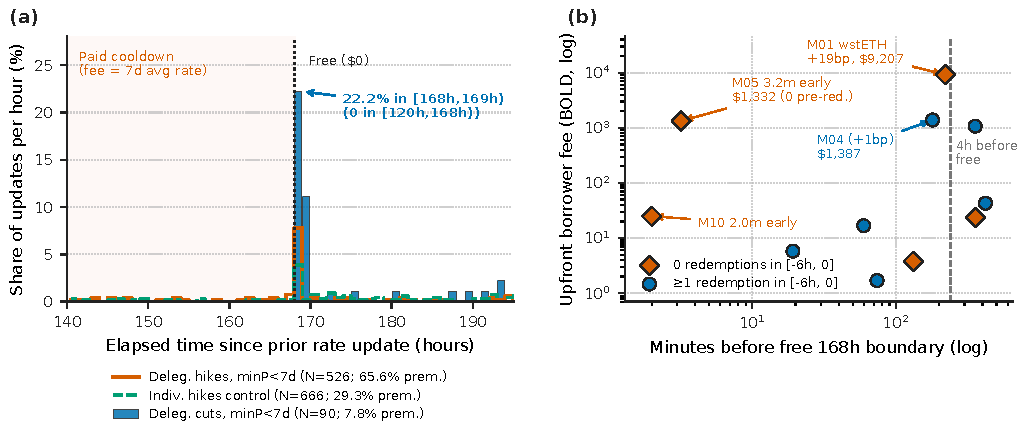
\includegraphics[width=0.98\textwidth]{figures/fig1_notch_bunching_agency.pdf}
\caption{Cooldown notch bunching at 168~hours and dominated near-notch delegated hikes. Panel~(a) plots hourly update density around the 168-hour fee cliff for managers facing the economic fee notch ($\text{minInterestRateChangePeriod} < 604{,}800$~s) alongside self-managed individual hikes, separating hardcoded 604,800-second revert walls. Panel~(b) maps paid positive-debt delegated hikes in $[160\text{h}, 168\text{h})$ by remaining minutes before free expiry (log scale) and borrower penalty (log BOLD), distinguishing events with zero branch redemptions in $[-6\text{h}, 0]$ (vermillion diamonds) from those with at least one prior redemption (navy circles).}
\label{fig:notch}
\end{figure}

\subsection{Dominated near-notch hikes and fee-base expansion}\label{subsec:dominated}

The agency wedge becomes unmistakable in the final four hours before cooldown expiry, where waiting minutes eliminates 100\% of the upfront penalty. Panel B of Table~\ref{tab:notch_agency} and Figure~\ref{fig:notch}(b) audit every single positive-debt delegated hike executed in $[164\text{h}, 168\text{h})$. Across the 485-day ledger, managers executed eight such hikes costing borrowers 11,979.39~BOLD (eleven hikes totaling 13,115.89~BOLD inside $[160\text{h}, 168\text{h})$). Live permission checks confirm that zero of the eight events hit \texttt{maxInterestRate}. Four of the eight hikes, accounting for 10,567.89~BOLD (88.2\% of near-notch fees), took place with exactly zero branch redemptions during both the six hours preceding the transaction and the six hours following it.

Three flagship episodes illustrate the magnitude of this borrower loss. On July 29, 2026 (Confirmation), manager M05 on wstETH (1.28~million~BOLD debt) raised its rate by 10~bp (5.20\% to 5.30\%) exactly 3.2~minutes before free cooldown expiry, charging borrowers 1,331.98~BOLD (54.4~times the 7-day value of the rate increment) while sitting inside the $[0.8\%, 71.7\%]$ tied-rate queue block with zero redemptions in $[-6\text{h}, +6\text{h}]$; justifying that fee at a 2\% disruption cost would require an annualized redemption arrival rate exceeding 8,500~per year. On October 18, 2025, manager M04 on wstETH (1.55~million~BOLD debt) paid 1,387.26~BOLD 179.6~minutes before free expiry for a single 1~bp rate step (4.61\% to 4.62\%) from a well-buffered queue interval of $[62.5\%, 67.6\%]$; under $\DesignAStar$, that 1~bp step would have cost 2.98~BOLD, a 99.8\% fee reduction. One week later on October 25, 2025, manager M01 on wstETH (10.07~million~BOLD debt) hiked 19~bp (4.61\% to 4.80\%) 220.4~minutes early from queue interval $[14.5\%, 47.5\%]$ with zero redemptions in $[-6\text{h}, +6\text{h}]$, capitalizing 9,207.19~BOLD onto borrower debt. On March 9, 2026, manager M10 on rETH paid 24.96~BOLD exactly 2.0~minutes before free expiry with zero redemptions in $[-24\text{h}, +24\text{h}]$.

Finally, we quantify the direct contractual fee-base expansion from capitalizing upfront penalties into \texttt{newDebt}. Capitalizing 411,349.00~BOLD across all 345 paid positive-debt premature hikes permanently raised managers' annualized management-fee income by $+1{,}159.82$~BOLD per year ($+1{,}191.72$~BOLD per year including the seven paid premature cuts totaling 10,637.60~BOLD). Although small relative to total management revenue (implying a conservative revenue-expansion wedge $\mu_{\text{pv}} \approx 0.0028$ in Section~\ref{sec:structural}), the sign of the contractual incentive runs directly opposite to borrower welfare: every dollar of capitalized upfront penalty adds to the manager's fee-earning principal.

\section{Mainnet spike-and-cut exploits and fee-rule replays}\label{sec:exploits}

\subsection{Forensic anatomy of live spike-and-cut reversals}\label{subsec:spike_cut}

The fixed branch-average cooldown fee in \eqref{eq:sq_fee} creates two opposite distortions. On small upward staircases, it steeply overcharges borrowers; on sharp temporary spikes followed by quick reversals, it systematically undercharges them. Whenever a manager sits outside cooldown ($\Delta t \ge 168\text{h}$), raising the batch rate to an arbitrarily high shield level $r_{\text{high}}$ costs 0.00~BOLD. Reversing back down to $r_{\text{low}}$ after $\Delta t \in (0, P)$ incurs only $D \bar{r} P / Y$, which falls below the honest 7-day excess holding cost $D (r_{\text{high}} - r_{\text{low}}) P / Y$ as soon as $r_{\text{high}} - r_{\text{low}} > \bar{r} P / (P - \Delta t)$.

Both live exploits break baseline $\DesignA$ as well. Scanning all 1,712 batch updates across 485~days identifies five premature spike-and-cut reversals (four in Development and one in Confirmation). Two episodes are strictly profitable under Status Quo, extracting 14,650.66~BOLD in combined arbitrage discounts relative to honest 7-day holding, while three episodes are profitable under naive increment-only $\DesignA$. Zero episodes profit under $\DesignAStar$ or $\DesignD$.

\begin{table}[!htbp]
\centering
\caption{Mainnet spike-and-cut arbitrage episodes and four-mechanism counterfactual fee replays.}
\label{tab:spike_mechanisms}
\footnotesize
\setlength{\tabcolsep}{4pt}
\resizebox{\textwidth}{!}{\begin{tabular}{@{}llrrrrrrrr@{}}
\toprule
\multicolumn{10}{@{}l}{\textit{Panel A: All five premature batch spike-and-cut reversals on Ethereum mainnet (485~days)}} \\
\midrule
Date / Branch / Mgr & Debt & Rate path & $\Delta t$ & 7d hold & SQ cut & SQ disc.\ & Cut vs.\ 7d & $\DesignAStar$ & $\DesignD$ \\
(Sample) & (M BOLD) & (\%) & (h) & (BOLD) & (BOLD) & (\%) & (\%) & fee / disc. & forf.\ / disc. \\
\midrule
2026-03-06 wstETH M01 (Dev) & 7.98 & $0.7\to 10.5\to 0.7$ & 1.01 & 15,001 & 2,307 & 84.02\% & 84.62\% & 14,911 / 0.0\% & 14,911 / 0.0\% \\
2026-03-06 WETH M03 (Dev) & 1.79 & $3.1\to 13.1\to 3.3$ & 1.01 & 3,357 & 1,291 & 60.96\% & 61.56\% & 3,337 / 0.0\% & 3,337 / 0.0\% \\
2026-08-25 wstETH M01 (Conf) & 7.79 & $6.0\to 6.3\to 0.7$ & 48.41 & 8,370 & 4,774 & $-96.22\%$ & 42.97\% & 5,958 / $-5.3\%$ & 5,898 / 0.0\% \\
2026-06-16 rETH M02 (Dev) & 3.83 & $2.7\to 8.7\to 3.0$ & 48.00 & 4,188 & 2,263 & $-127.99\%$ & 45.98\% & 2,992 / $-106.1\%$ & 3,017 / 0.0\% \\
2025-06-22 wstETH M04 (Dev) & 0.002 & $3.21\to 3.41\to 3.31$ & 76.38 & 0.04 & 1.34 & $-3410\%$ & $-3365\%$ & 0.02 / 0.0\% & 0.02 / 0.0\% \\
\midrule
\multicolumn{10}{@{}l}{\textit{Panel B: Exact four-mechanism counterfactual fee replay across Development, Confirmation, and Pooled splits}} \\
\midrule
Sample & Status Quo & \multicolumn{2}{c}{Baseline $\DesignA$} & \multicolumn{2}{c}{$\DesignAStar$ (0 slots)} & \multicolumn{2}{c}{$\DesignD$ (1-slot)} & \multicolumn{2}{c}{$\DesignAStar$ / $\DesignD$ saved} \\
(Updates; paid; staircase) & (BOLD; /M-dd) & \multicolumn{2}{c}{(BOLD; /M-dd)} & \multicolumn{2}{c}{(BOLD; /M-dd)} & \multicolumn{2}{c}{(BOLD; /M-dd)} & \multicolumn{2}{c}{(\% vs.\ SQ)} \\
\midrule
Development (408d) & 318,054.00 & \multicolumn{2}{c}{34,837.53} & \multicolumn{2}{c}{50,218.68} & \multicolumn{2}{c}{21,377.67} & \multicolumn{2}{c}{$-84.2\%$ / $-93.3\%$} \\
\quad (1,268; 292; 254) & (57.96 /M-dd) & \multicolumn{2}{c}{(6.35 /M-dd)} & \multicolumn{2}{c}{(9.15 /M-dd)} & \multicolumn{2}{c}{(3.88* /M-dd)} & \multicolumn{2}{c}{[48.81 / 54.09 /M-dd]} \\
Confirmation (77d) & 103,932.60 & \multicolumn{2}{c}{17,023.85} & \multicolumn{2}{c}{18,208.60} & \multicolumn{2}{c}{5,949.23} & \multicolumn{2}{c}{$-82.5\%$ / $-94.3\%$} \\
\quad (372; 60; 54) & (78.64 /M-dd) & \multicolumn{2}{c}{(12.88 /M-dd)} & \multicolumn{2}{c}{(13.78 /M-dd)} & \multicolumn{2}{c}{(4.46* /M-dd)} & \multicolumn{2}{c}{[64.87 / 74.18 /M-dd]} \\
Pooled (485d) & 421,986.60 & \multicolumn{2}{c}{51,861.37} & \multicolumn{2}{c}{68,427.29} & \multicolumn{2}{c}{27,326.90} & \multicolumn{2}{c}{$-83.8\%$ / $-93.5\%$} \\
\quad (1,640; 352; 308) & (61.98 /M-dd) & \multicolumn{2}{c}{(7.62 /M-dd)} & \multicolumn{2}{c}{(10.05 /M-dd)} & \multicolumn{2}{c}{(3.99* /M-dd)} & \multicolumn{2}{c}{[51.93 / 57.99 /M-dd]} \\
\bottomrule
\end{tabular}}
\par\vspace{4pt}\begin{minipage}{\textwidth}\footnotesize\setlength{\parskip}{0pt}\textit{Notes.} Panel A reports every premature batch reversal following a rate spike across all 1,712 canonical batch updates. SQ disc.\ equals $1 - (\text{hike fee} + \text{spike excess interest} + \text{cut fee}) / \text{7d hold excess}$; Cut vs.\ 7d compares the cut fee alone to 7-day excess holding cost (alternative cut-fee vs.\ remaining-cooldown ratios are 84.53\% on M01 and 61.33\% on M03). Under baseline $\DesignA$, the 2026-08-25 wstETH M01 episode turns $+8.85\%$ profitable because the initial premature hike fee drops while the cut fee remains capped at $\bar{r}$. Under $\DesignAStar$, signed total-excess discounts equal 0.000\% on free-spike episodes (rows 1, 2, 5) and are strictly negative ($-5.30\%$ and $-106.14\%$) on premature-hike reversals (rows 3--4) because both the upward increment and downward commitment fees apply, leaving zero positive arbitrage gain ($\max(0, \text{disc.}) = 0.0\%$) across all five episodes. Panel B replays all genuine changed updates on exact pre-update state; $\DesignD$ totals equal forfeited escrow plus 5\% annual opportunity cost on exact locked BOLD-days (107.84~BOLD Dev, 50.81~BOLD Conf, 158.65~BOLD Pooled; asterisked per-M-dd values denote forfeited escrow excluding opportunity cost), with 0 escrow underflows across all 1,712 mainnet updates.
\end{minipage}
\end{table}

Panel A of Table~\ref{tab:spike_mechanisms} and Figure~\ref{fig:exploits}(a) dissect all five reversals. The two live exploits occurred simultaneously on March 6, 2026 between 15:50:47 and 16:51:23~UTC, lasting 3,636~seconds (1.01~hours, just past the 1-hour \texttt{MIN\_INTEREST\_RATE\_CHANGE\_PERIOD} floor). On wstETH, manager M01 (controlling 7,981,790.37~BOLD of pooled debt) executed a free post-cooldown spike from 0.70\% to 10.50\% (+980~bp) and reversed straight back to 0.70\% one hour later. Holding 10.50\% for seven full days would have cost borrowers 15,001.39~BOLD in excess interest. Instead, M01 paid 90.19~BOLD in excess interest during the 1.01-hour shield window plus a Status Quo cut fee of 2,307.13~BOLD, totaling 2,397.31~BOLD, an 84.02\% total-excess arbitrage discount (84.53\% comparing the cut fee to remaining-cooldown interest; 84.62\% comparing the cut fee to full 7-day interest) and 12,604.08~BOLD in avoided commitment cost. At the exact same block timestamps on WETH, manager M03 (1,786,300.65~BOLD debt) spiked freely from 3.10\% to 13.10\% (+1,000~bp) and cut back to 3.30\%, paying 20.18~BOLD in excess interest plus 1,290.50~BOLD in cut fees against a 3,357.27~BOLD honest 7-day excess hold, a 60.96\% total-excess discount (61.33\% versus remaining hold; 61.56\% versus 7-day hold) saving 2,046.58~BOLD.

The Confirmation episode on August 25--27, 2026 exposes a subtle failure mode of naive incremental reforms. When M01 on wstETH (7.79~million~BOLD debt) stepped up prematurely from 6.00\% to 6.30\% and then slashed to 0.70\% 48.41~hours later, the episode was unprofitable under Status Quo ($-96.22\%$ total-excess discount) only because Status Quo taxed the initial 30~bp hike at the full branch average. Under baseline $\DesignA$, that 30~bp upward hike fee collapses to a tiny incremental charge while the 560~bp downward cut fee stays capped at $\bar{r}$, flipping the episode into an $+8.85\%$ profitable arbitrage. Under $\DesignAStar$ \eqref{eq:design_astar}, the downward commitment fee rises automatically to $D(r_0 - r_1)(P - \Delta t)/Y$ (14,911.21~BOLD on M01 wstETH, 3,337.08~BOLD on M03 WETH, and 5,958.44~BOLD on the Confirmation reversal); this matches the honest 7-day holding cost to the cent on free-spike episodes (0.000\% discount) while imposing strictly negative signed discounts ($-5.30\%$ and $-106.14\%$) on premature-hike reversals where both upward and downward fees apply, so positive arbitrage gain drops to 0.000\% on every episode. Hardened $\DesignD$ delivers identical zero-arbitrage forfeitures (14,911.02, 3,337.03, and 5,898.42~BOLD).

\subsection{Proactive audit of batch-join and switch bypass paths}\label{subsec:batch_transitions}

Smart-contract rate transitions do not flow exclusively through direct rate-update calls. In deployed Liquity V2 \texttt{BorrowerOperations}, a borrower can alter her effective interest rate through four distinct entry points: individual rate adjustment (\texttt{op=3}), batch rate adjustment (\texttt{BatchUpdated}), batch removal (\texttt{op=8}), and joining or switching into a lower-rate batch (\texttt{op=7} and \texttt{op=9}). As shown in \citet{companion2026}, if a protocol patches only individual and batch rate updates with $\DesignAStar$ while leaving batch joins and switches under Status Quo fees, an adversary can execute a free post-cooldown spike from 0.5\% to 250\% and switch one block later into a 0.5\% batch, capturing a 98.60\% bypass with zero flash loans.

To assess whether mainnet participants have already exploited this vector, we replay exact pre-operation trove snapshots across every batch join, removal, and switch in our 485-day ledger (304 joins under \texttt{op=7}, 102 removals under \texttt{op=8}, and 75 switches under \texttt{op=9}). Sixty-four of those 481 transitions lowered the borrower's effective interest rate, and 17 occurred within seven days of a prior upward rate change or opening (2 following an individual \texttt{op=3} hike, 7 following an individual \texttt{op=0} trove opening, and 8 following a \texttt{BatchUpdated} manager hike). No mainnet borrower exploited this bypass vector. Across all 17 within-7-day transitions, zero yielded a positive arbitrage discount relative to 7-day holding; the closest case (a Confirmation \texttt{op=9} switch out of manager M17 on wstETH from 6.0\% to 0.5\% after 73.97~hours on 241,018~BOLD debt) posted a $-0.58\%$ discount. Guarding all four contract entry points under $\DesignAStar$ and $\DesignD$ therefore closes an unexploited zero-day vulnerability proactively before malicious bots weaponize it.

\subsection{Four-mechanism counterfactual replays}\label{subsec:replays}

We next measure the exact fixed-action statutory fee savings across all four mechanisms (Status Quo, baseline $\DesignA$, $\DesignAStar$, and hardened one-slot $\DesignD$) on all 1,640 genuine batch rate updates, reserving endogenous equilibrium best-response adjustments for Section~\ref{sec:structural}. Under Status Quo, 308 paid staircase hikes (254 in Development and 54 in Confirmation) account for 93.73\% (395,542.67~BOLD) of all 421,986.60~BOLD in batch repricing penalties (93.64\% in Development; 94.03\% in Confirmation). Microstructure diagnostics confirm why Status Quo is so punitive: across all 308 staircase hikes, the median rate increment is just 20.0~bp (IQR $[10.0, 30.0]$~bp) at a median elapsed time of 41.22~hours, producing a median Status Quo to $\DesignAStar$ overcharge ratio of 20.79~times (10.99~times dollar-weighted).

\begin{figure}[!htbp]
\centering
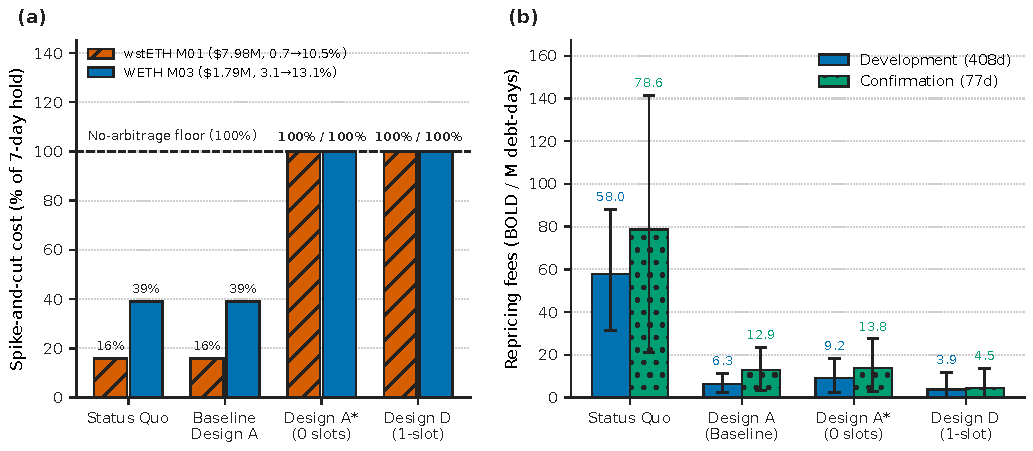
\includegraphics[width=0.98\textwidth]{figures/fig2_spike_cut_and_mechanisms.pdf}
\caption{Mainnet spike-and-cut arbitrage vulnerability and counterfactual repricing-fee replays. Panel~(a) compares total spike-and-cut excess cost as a share of honest 7-day holding cost across all four fee rules for the live March 6, 2026 wstETH M01 (7.98M~BOLD) and WETH M03 (1.79M~BOLD) episodes; the dashed line marks the 100\% no-arbitrage floor. Panel~(b) plots exact fixed-action repricing fees in BOLD per million debt-days with 14-day circular block-bootstrap 95\% confidence intervals across Development (408~days) and Confirmation (77~days).}
\label{fig:exploits}
\end{figure}

Panel B of Table~\ref{tab:spike_mechanisms} and Figure~\ref{fig:exploits}(b) report exact replays across Development, Confirmation, and Pooled samples. Replacing Status Quo with zero-storage $\DesignAStar$ slashes pooled repricing penalties by 83.78\% ($-353{,}559.31$~BOLD), from 421,986.60~BOLD (61.98~BOLD/M debt-days, 95\% CI $[38.33, 90.11]$) down to 68,427.29~BOLD (10.05~BOLD/M debt-days, $[4.04, 17.45]$), saving 51.93~BOLD/M debt-days (95\% CI $[28.25, 78.10]$). Savings hold tightly out of sample: $-84.21\%$ in Development (57.96 to 9.15~BOLD/M debt-days) and $-82.48\%$ in Confirmation (78.64 to 13.78~BOLD/M debt-days). Relative to naive baseline $\DesignA$ (51,861.37~BOLD pooled), $\DesignAStar$ collects 16,565.91~BOLD more on premature downward cuts (27,203.51 versus 10,637.60~BOLD), the exact commitment clawback needed to defeat spike-and-cut arbitrage while leaving upward staircase savings intact (359,554.79~BOLD saved on staircases alone).

Hardened one-slot $\DesignD$ cuts borrower fees even further while closing flash-loan close-and-reopen exploits. Because honest rate hikes that are held for seven days vest 100\% of their locked escrow back to borrowers, total forfeited escrow across 485~days falls to 27,168.26~BOLD (3.99~BOLD/M debt-days; 21,269.84~BOLD Development and 5,898.42~BOLD Confirmation). Zero escrow underflows occur across 1,712 updates. By contrast, a deprecated high-water-rate formulation triggers three mainnet underflows. Accounting for the exact locked escrow balance (1,158,131.46~BOLD-days pooled, averaging just 2,387.90~BOLD across the entire protocol at any instant) at a 5\% annual capital opportunity cost adds only 158.65~BOLD over 485~days, yielding an all-in $\DesignD$ cost of 27,326.90~BOLD, a 93.52\% reduction ($-394{,}659.70$~BOLD; $-93.28\%$ Development and $-94.28\%$ Confirmation).

\section{Causal identification via mechanical routing and cross-manager leapfrogging}\label{sec:causal}

\subsection{Mechanical CollateralRegistry routing and within-trove responses}\label{subsec:routing}

Descriptive regressions comparing delegated and self-managed troves cannot rule out borrower self-selection: borrowers who expect heavy redemption risk or who monitor less frequently may voluntarily select into delegated pools. To isolate causal responsiveness to redemption pressure without relying on voluntary delegation timing, we exploit an exact institutional rule hardcoded inside Liquity V2's \texttt{CollateralRegistry}. Every time an arbitrageur redeems BOLD for collateral, the contract partitions the redemption across WETH, wstETH, and rETH strictly in proportion to each branch's unbacked debt ($U_{b,t} = D_{b,t} - \text{SP}_{b,t}$), where $\text{SP}_{b,t}$ is that branch's Stability Pool BOLD balance. When Stability Pool depositors migrate across branches chasing yield or collateral liquidation preferences, a branch's mechanical routing share $s_{b,t} = U_{b,t} / \sum_{b'} U_{b',t}$ swings wildly even when aggregate BOLD peg demand and ETH prices are unchanged.

Offline reconstruction recovers exact branch routing shares from 1,708 multi-branch redemption transactions out of 1,709 canonical redemption transactions (1,223 hitting all three branches and 485 hitting two branches across 255 active redemption days). Routing shares swing 100-fold across collateral branches. Figure~\ref{fig:causal}(a) displays these mechanical shifts. In May 2025, WETH absorbed 70.35\% of protocol redemptions while wstETH took 24.02\% and rETH took 5.63\%. By spring 2026 (March through May 2026), abundant WETH Stability Pool deposits drove WETH's unbacked debt near zero, collapsing its routing share to 0.00\% in March and 1.16\% across the three-month shutdown window (8,756~BOLD total redemptions, triggering exactly zero WETH staircase hikes), while wstETH absorbed 88.14\% (peaking at 97.53\% in May 2026). Once Stability Pool balances rebalanced in summer 2026, WETH's routing share rebounded to 31.75\% in July and 45.83\% in August.

We first embed these routing swings inside our daily loan-level panel ($N = 72{,}070$ Development, $13{,}607$ Confirmation, $85{,}677$ Pooled loan-days) with Trove fixed effects ($\gamma_i$) and Branch-by-Day fixed effects ($\delta_{b,t}$):
\begin{equation}\label{eq:trove_fe}
r_{i,b,t} = \gamma_i + \delta_{b,t} + \beta_0\,\text{Delegated}_{i,t} + \beta_1\bigl(\text{Delegated}_{i,t} \times s_{b,t}\bigr) + \beta_2 \log(\text{debt}_{i,b,t}) + \varepsilon_{i,b,t},
\end{equation}
clustering standard errors two-way by trove and calendar day. Because $\delta_{b,t}$ absorbs all branch-specific macro shocks, collateral yield differentials, and daily market clearing rates, $\beta_1$ identifies whether delegated troves hike base rates more aggressively than self-managed troves inside the same branch on days when mechanical routing concentrates redemption pressure on that branch. To eliminate any contemporaneous feedback between borrower rate changes and same-day Stability Pool flows, our preferred specification replaces $s_{b,t}$ with the predetermined trailing 7-day average routing share $\bar{s}_{b,t-1}^{(7)} = \frac{1}{7}\sum_{\ell=1}^{7} s_{b,t-\ell}$.

Panel A of Table~\ref{tab:causal_routing} reports the panel estimates. In Development, delegated loans increase quoted base rates by $+95.87$~bp per unit of contemporaneous routing share ($\text{SE} = 27.90$, $p = 0.0006$; equal-weighted $+72.30$~bp, $p = 0.0058$) and by $+110.04$~bp using predetermined trailing 7-day average routing share ($\text{SE} = 31.05$, $p = 0.0004$), while quoting $-101.25$~bp below unbatched loans at zero routing exposure ($p = 0.0029$). Across the pooled 485-day panel, the predetermined lagged interaction remains positive and statistically significant at the 5\% level ($+73.06$~bp, $\text{SE} = 35.18$, $p = 0.0378$; contemporaneous $+60.45$~bp, $p = 0.0978$). Transparently, the short 77-day Confirmation holdout has muted cross-branch routing spread and wide standard errors ($+34.84$~bp contemporaneous, $\text{SE} = 166.04$, $p = 0.834$; $+64.61$~bp lagged, $p = 0.649$; equal-weighted $-106.65$~bp, $p = 0.154$).

\subsection{Predetermined Bartik shift-share instrumental variables}\label{subsec:bartik}

To identify the direct causal impact of redemption waves on delegated upfront repricing fees, we construct a predetermined Bartik shift-share instrument \citep{borusyak2022quasi} combining each branch's predetermined trailing 7-day average mechanical routing share $\bar{s}_{b,t-1}^{(7)}$ with leave-branch-out protocol-wide redemption volume $R_{-b,t}$:
\begin{equation}\label{eq:bartik_iv}
Z_{b,t}^{\text{Bartik}} = \log\!\bigl(1 + \bar{s}_{b,t-1}^{(7)}\,R_{-b,t}\bigr).
\end{equation}
The exclusion restriction relies on quasi-random assignment of daily macro peg-arbitrage inflows $R_{-b,t}$ across branches predetermined over the preceding seven days by Stability Pool deposit balances, conditional on Branch fixed effects ($\alpha_b$), Day fixed effects ($\lambda_t$), and the linear lagged-share control $\bar{s}_{b,t-1}^{(7)}$. Because \texttt{CollateralRegistry} routing is deterministic in bytecode, the first stage predicting realized log branch redemption volume $\log(1 + R_{b,t})$ is powerful across every sample. We compute 2SLS estimates with exact fixed-effect degrees-of-freedom (FE-DOF) standard errors clustered by calendar day, Driscoll--Kraay serial-correlation-adjusted standard errors ($L = 2$ and $L = 7$ days) \citep{driscoll1998consistent}, and 499-draw 14-day circular block-bootstrap confidence intervals.

\begin{table}[!htbp]
\centering
\caption{Causal identification of delegated rate and fee responses via \texttt{CollateralRegistry} routing.}
\label{tab:causal_routing}
\footnotesize
\setlength{\tabcolsep}{4.5pt}
\resizebox{\textwidth}{!}{\begin{tabular}{@{}llrrrrrr@{}}
\toprule
Specification and outcome & Sample & $N$ & First-stage $F$ & Coeff.\ & FE-DOF SE & $p$-value & Serial-adj.\ / Boot CI \\
\midrule
\multicolumn{8}{@{}l}{\textit{Panel A: Loan-day panel with Trove FE + Branch $\times$ Day FE (base APR in bp, two-way clustered)}} \\
$\text{Delegated} \times s_{b,t}$ (debt-weighted) & Dev & 72,070 & -- & $+95.87$ & 27.90 & 0.0006 & EQW $+72.30$ ($p=0.006$) \\
$\text{Delegated} \times s_{b,t}$ (debt-weighted) & Conf & 13,607 & -- & $+34.84$ & 166.04 & 0.8338 & EQW $-106.65$ ($p=0.154$) \\
$\text{Delegated} \times s_{b,t}$ (debt-weighted) & Pooled & 85,677 & -- & $+60.45$ & 36.51 & 0.0978 & EQW $+41.07$ ($p=0.080$) \\
$\text{Delegated} \times \bar{s}_{b,t-1}^{(7)}$ (predet.\ 7d avg) & Dev & 72,070 & -- & $+110.04$ & 31.05 & 0.0004 & Base at $s=0$: $-101.25$ \\
$\text{Delegated} \times \bar{s}_{b,t-1}^{(7)}$ (predet.\ 7d avg) & Conf & 13,607 & -- & $+64.61$ & 142.14 & 0.6494 & Base at $s=0$: $+52.00$ \\
$\text{Delegated} \times \bar{s}_{b,t-1}^{(7)}$ (predet.\ 7d avg) & Pooled & 85,677 & -- & $+73.06$ & 35.18 & 0.0378 & Base at $s=0$: $-69.11$ \\
\addlinespace[4pt]
\multicolumn{8}{@{}l}{\textit{Panel B: Branch-day Bartik shift-share 2SLS (Branch FE + Day FE; 48h upfront fee in BOLD/M debt-days)}} \\
48h upfront fee (\texttt{fee\_mdd\_48h}) & Dev & 1,220 & 150.0 & $+10.53$ & 6.96 & 0.1303 & Boot $[-1.57, +31.27]$ \\
48h upfront fee (\texttt{fee\_mdd\_48h}) & Conf & 231 & 41.1 & $+20.34$ & 12.19 & 0.0954 & Boot $[-19.62, +265.19]$ \\
48h upfront fee (\texttt{fee\_mdd\_48h}) & Pooled & 1,451 & 197.7 & $+13.53$ & 6.41 & 0.0347 & Boot $[+2.78, +35.02]$ \\
\quad Driscoll--Kraay $L=2$ / $L=7$ & Pooled & 1,451 & 197.7 & $+13.53$ & 7.74 & 0.0810 & $L=7$ SE 7.84 ($p=0.085$) \\
24h non-overlapping fee (\texttt{fee\_mdd}) & Pooled & 1,451 & 197.7 & $+4.76$ & 3.98 & 0.2309 & Boot $[-1.73, +14.79]$ \\
Placebo lead $t+7\text{d}$ (Wald-scaled) & Pooled & 1,425 & 197.7 & $+3.58$ & 8.25 & 0.6644 & Null pre-trend pass \\
\addlinespace[4pt]
\multicolumn{8}{@{}l}{\textit{Panel C: All-21 positive-debt manager panel Bartik 2SLS (Manager $\times$ Branch FE + Day FE; 48h fee/M-dd)}} \\
48h upfront fee (\texttt{fee\_mdd\_48h}) & Dev & 4,127 & 151.4 & $+23.11$ & 15.53 & 0.1479* & DK $L=2$ $p=0.1075$ \\
48h upfront fee (\texttt{fee\_mdd\_48h}) & Conf & 934 & 171.3 & $+24.44$ & 11.71 & 0.0369 & $p_t=0.0522$; DK $p=0.195$ \\
48h upfront fee (\texttt{fee\_mdd\_48h}) & Pooled & 5,061 & 241.1 & $+29.71$ & 15.30 & 0.0522 & $p_t=0.0616$; DK $p=0.0374$ \\
\bottomrule
\end{tabular}}
\par\vspace{4pt}\begin{minipage}{\textwidth}\footnotesize\setlength{\parskip}{0pt}\textit{Notes.} Panel A estimates \eqref{eq:trove_fe} on daily loan snapshots with Trove and Branch $\times$ Day fixed effects plus $\log(\text{debt}_{i,b,t})$, clustering standard errors two-way by trove and calendar day (EQW denotes equal-weighted checks). Panel B estimates Branch-Day 2SLS using the predetermined Bartik shift-share instrument \eqref{eq:bartik_iv} and linear control $\bar{s}_{b,t-1}^{(7)}$ with exact fixed-effect degrees-of-freedom (FE-DOF) standard errors clustered by day, Driscoll--Kraay (DK) $L=2$ and $L=7$ serial-correlation-adjusted SEs, and 499-draw 14-day circular block-bootstrap 95\% CIs; forward leads and lags are constructed strictly inside each split. Panel C extends the debt-weighted Bartik 2SLS design (including linear $\bar{s}_{b,t-1}^{(7)}$ control) to all 21 distinct positive-debt managers (31 manager-branch pairs pooled; 19 managers in Development and 14 in Confirmation) with Manager $\times$ Branch FE and Day FE (two-way clustered by manager-branch and day; asterisked Dev $p=0.1479$ uses cluster $t$-df; normal $p=0.1368$).
\end{minipage}
\end{table}

Panel B of Table~\ref{tab:causal_routing} and Figure~\ref{fig:causal}(b) summarize the Bartik 2SLS evidence. First-stage $F$-statistics reach 150.0 in Development, 41.1 in Confirmation, and 197.7 Pooled (first-stage slope $\hat{\pi} = 0.921$, $t = 14.06$). A one-unit increase in log branch redemption volume causally raises delegated 48-hour upfront repricing fees by $+10.53$~BOLD per million debt-days in Development ($\text{SE} = 6.96$, $p = 0.130$), $+20.34$ in Confirmation ($\text{SE} = 12.19$, $p = 0.095$), and $+13.53$~BOLD per million debt-days Pooled (FE-DOF day-clustered $\text{SE} = 6.41$, $p = 0.0347$; cluster $t$-distribution $p = 0.0352$; Driscoll--Kraay $L = 2$ $\text{SE} = 7.74$, $p = 0.0810$; 14-day block-bootstrap 95\% CI $[+2.78, +35.02]$). Future placebo leads are cleanly null. Regressing 48-hour upfront fees on the 7-day-ahead future instrument yields a matched Wald-scaled placebo of $+3.58$ ($\text{SE} = 8.25$, $p = 0.664$). Zero anticipatory pre-trends appear in the data. Panel C extends the debt-weighted Bartik 2SLS design to the granular manager-branch-day panel covering all 21 positive-debt managers (31 manager-branch pairs pooled; 19 managers in Development and 14 in Confirmation; $N = 5{,}061$, Manager $\times$ Branch FE + Day FE, $F = 241.1$), delivering consistent positive fee responses of $+23.11$ in Development ($p_t = 0.148$), $+24.44$ in Confirmation (normal $p = 0.0369$, $p_t = 0.0522$), and $+29.71$~BOLD per million debt-days Pooled (normal $p = 0.0522$, $p_t = 0.0616$, Driscoll--Kraay $L = 2$ $p = 0.0374$).

Four boundary diagnostics clarify exactly where statistical power resides. First, non-overlapping 24-hour fee responses (\texttt{fee\_mdd}, $+4.76$, $p = 0.231$) and unweighted binary hike-count 2SLS regressions lack precision because major repricing waves unfold across 24--48~hours on large multi-million-dollar batches. Second, pure external market instruments interacting lagged routing share with BOLD secondary-market depeg or ETH volatility exhibit weak first stages ($z_{\text{depeg}}$ $F = 9.36$, $z_{\text{vol}}$ $F = 0.76$), rendering their 2SLS point estimates noisy. Third, an exploratory positive-debt-only specification with Manager $\times$ Day fixed effects restricts the sample to 1,041 observations where only two managers (M08 and M10) hold simultaneous positive debt across all three branches, yielding positive OLS ($+2.45$~pp 48-hour hike probability, $p = 0.154$; $+15.01$ fee/M-dd, $p = 0.123$) and an underpowered Bartik 2SLS ($+1.39$~pp, $p = 0.400$; $+17.07$ fee/M-dd, $p = 0.349$). Taken together, the routing natural experiment identifies economically large causal fee responses concentrated in heavy-debt multi-day redemption waves.

\begin{figure}[!htbp]
\centering
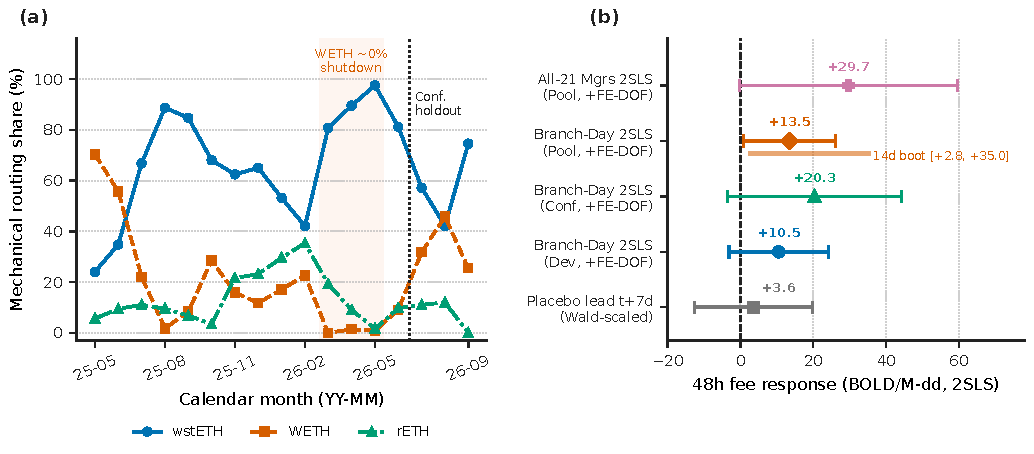
\includegraphics[width=0.98\textwidth]{figures/fig3_causal_routing_did.pdf}
\caption{Mechanical \texttt{CollateralRegistry} routing swings and predetermined Bartik shift-share 2SLS estimates. Panel~(a) tracks monthly mean unbacked-debt routing shares reconstructed from 1,708 multi-branch redemption transactions, shading the March--May 2026 WETH near-zero routing shutdown and marking the July 1, 2026 Confirmation holdout boundary. Panel~(b) displays FE-DOF 2SLS 48-hour upfront fee responses (BOLD per million debt-days) with 95\% confidence intervals across Development, Confirmation, Pooled branch-day, all-21 manager panels, the 14-day block-bootstrap interval, and the matched Wald-scaled $t+7\text{d}$ placebo lead.}
\label{fig:causal}
\end{figure}

\subsection{Multivariate Hawkes estimation of cross-manager leapfrogging}\label{subsec:hawkes}

Mechanical routing shocks explain why redemptions trigger manager rate hikes, yet descriptive timing evidence points to a second amplifier: strategic cross-manager escalation. Across all 1,640 genuine pooled batch updates, 2,188 cross-manager pairs occur within two hours inside the same collateral branch (1,937 within one hour), and 93.83\% of those two-hour pairs move in the exact same direction (1,742 simultaneous hikes and 311 simultaneous cuts; 94.84\% within one hour, binomial $p < 10^{-100}$). Tracking cross-manager rate crossings inside seven-day windows uncovers 4,472 leapfrog reversals involving 870 retaliation hikes (median retaliation latency 48.66~hours) and 385,840.34~BOLD in retaliation hike penalties.

Simultaneous hikes alone could reflect rapid parallel reactions to a shared external redemption event. To separate genuine rival-to-rival leapfrogging from common shocks, we estimate a marked multivariate Hawkes point-process model \citep{hawkes1971spectra,ogata1988statistical} for positive-debt manager rate hikes in each branch and sample split. For manager $m \in \{1, \dots, M\}$ in branch $b$, instantaneous hike intensity at continuous timestamp $t$ (in hours) obeys
\begin{equation}\label{eq:hawkes}
\begin{aligned}
\lambda_{m}(t) &= \pi_m\bigl(\mu_{\text{tot}} + \gamma_{\text{red}}\,\tilde{R}_b(t; \kappa_{\text{red}}) + \gamma_{\text{vol}}\,\tilde{V}(t)\bigr) \\
&\quad + \alpha_{\text{self}} \beta \sum_{t_k^{(m)} < t} e^{-\beta(t - t_k^{(m)})}
+ \frac{\alpha_{\text{cross}} \beta}{M - 1} \sum_{j \ne m} \sum_{t_k^{(j)} < t} e^{-\beta(t - t_k^{(j)})},
\end{aligned}
\end{equation}
where $\pi_m = N_m / N$ is manager $m$'s empirical hike share, $\tilde{R}_b(t; \kappa_{\text{red}})$ is the unit-time-average normalization on $[0, T]$ of $\sum_{\tau_\ell < t} \log(1 + \text{Red}_{\ell}/1{,}000)\,\kappa_{\text{red}}\,e^{-\kappa_{\text{red}}(t - \tau_\ell)}$, $\tilde{V}(t)$ captures realized ETH volatility normalized to unit time-average, $\alpha_{\text{self}} \ge 0$ is same-manager self-excitation, and $\alpha_{\text{cross}} \ge 0$ is cross-manager branching excitation with decay rate $\beta$ (half-life $t_{1/2} = \ln 2 / \beta$). To rule out the hardest competing hypothesis, namely that fast redemption bursts mimic rival contagion when $\kappa_{\text{red}}$ is fixed too slowly, we estimate a hostile free-$\kappa_{\text{red}}$ joint profile MLE allowing the exogenous redemption half-life to adjust freely from 0.5~minutes to 24~hours separately inside both the null model ($M_2$: $\alpha_{\text{cross}} = 0$) and the full model ($M_3$: $\alpha_{\text{cross}} \ge 0$). Every goodness-of-fit Kolmogorov--Smirnov (KS) statistic evaluates exact analytical piecewise Ogata time-rescaling integrals with zero numerical quadrature error.

\begin{table}[!htbp]
\centering
\caption{Multivariate Hawkes MLE and free-$\kappa_{\text{red}}$ cross-manager leapfrogging tests (positive-debt hikes).}
\label{tab:hawkes}
\footnotesize
\setlength{\tabcolsep}{4.2pt}
\resizebox{\textwidth}{!}{\begin{tabular}{@{}llrrrrrrrrr@{}}
\toprule
Sample & Branch & $N$ ($M$) & $\hat{\alpha}_{\text{self}}$ & $\hat{\alpha}_{\text{cross}}$ (SE) & $t_{1/2}$ (m) & Exact KS ($p$) & Free-$\kappa$ $\hat{\alpha}_{\text{cross}}$ & Free-$\kappa$ LRT ($p$) & Cross fee \% \\
\midrule
Dev & WETH & 82 (5) & 0.000 & 0.252 (0.057) & 11.04 & 0.109 (0.260) & 0.251 & 99.2 ($2.3\times 10^{-23}$) & 11.7\% \\
Dev & wstETH & 219 (10) & 0.000 & 0.411 (0.046) & 19.09 & 0.056 (0.486) & 0.408 & 312.2 ($7.3\times 10^{-70}$) & 22.8\% \\
Dev & rETH & 133 (7) & 0.091 & 0.451 (0.066) & 37.61 & 0.152 (0.004) & 0.445 & 162.6 ($3.0\times 10^{-37}$) & 31.8\% \\
\addlinespace[3pt]
Conf & WETH & 23 (5) & 0.000 & 0.167 (0.093) & 14.02 & 0.154 (0.590) & 0.176 & 13.1 ($2.9\times 10^{-4}$) & 19.7\% \\
Conf & wstETH & 58 (6) & 0.000 & 0.647 (0.107) & 6.65 & 0.231 (0.003) & 0.643 & 272.4 ($3.4\times 10^{-61}$) & 12.6\% \\
Conf & rETH & 20 (5) & 0.000 & 0.460 (0.158) & 10.67 & 0.105 (0.963) & 0.386 & 35.6 ($2.5\times 10^{-9}$) & 1.9\% \\
\addlinespace[3pt]
Pooled & WETH & 105 (7) & 0.000 & 0.230 (0.049) & 11.24 & 0.141 (0.028) & 0.229 & 95.7 ($1.4\times 10^{-22}$) & 10.9\% \\
Pooled & wstETH & 277 (11) & 0.000 & 0.455 (0.043) & 14.40 & 0.094 (0.014) & 0.450 & 495.2 ($1.1\times 10^{-109}$) & 18.7\% \\
Pooled & rETH & 153 (8) & 0.064 & 0.456 (0.060) & 30.21 & 0.133 (0.008) & 0.449 & 190.5 ($2.4\times 10^{-43}$) & 28.1\% \\
\bottomrule
\end{tabular}}
\par\vspace{4pt}\begin{minipage}{\textwidth}\footnotesize\setlength{\parskip}{0pt}\textit{Notes.} Estimates \eqref{eq:hawkes} by maximum likelihood on strictly positive-debt batch manager hikes across Development (408d), Confirmation (77d), and Pooled (485d) samples; $N$ counts events and $M$ active positive-debt managers. Exact KS reports the Kolmogorov--Smirnov statistic and p-value on exact analytical Ogata time-rescaled inter-arrival residuals. Free-$\kappa$ columns jointly profile the exogenous redemption-shock decay half-life from 0.5~min to 24~h inside both $M_2$ (null, $\alpha_{\text{cross}}=0$) and $M_3$ (full) and report the resulting likelihood-ratio statistic (LRT) against $M_2$. Cross fee \% is the share of positive-debt hike penalties attributed to cross-manager contagion via intensity decomposition (pooled aggregate across all branches: 89,543.95~BOLD, or 21.77\% of 411,349.00~BOLD; Development aggregate: 79,700.40~BOLD, or 25.53\%).
\end{minipage}
\end{table}

Cross-manager contagion survives every branch and sample. Table~\ref{tab:hawkes} and Figure~\ref{fig:hawkes} establish strong, out-of-sample leapfrogging across all six branch-samples. Even when the exogenous redemption shock adjusts freely across every branch-sample (optimal $M_3$ half-lives spanning 0.49~minutes on Confirmation WETH to 123.2~minutes on Development wstETH, and 0.49 to 10.68~minutes across Confirmation), cross-manager contagion remains large and statistically unmistakable in 6 of 6 branch-samples: Development WETH ($\hat{\alpha}_{\text{cross}} = 0.251$, LRT $= 99.2$, $p = 2.3 \times 10^{-23}$), Development wstETH ($\hat{\alpha}_{\text{cross}} = 0.408$, LRT $= 312.2$, $p = 7.3 \times 10^{-70}$), Development rETH ($\hat{\alpha}_{\text{cross}} = 0.445$, LRT $= 162.6$, $p = 3.0 \times 10^{-37}$), Confirmation WETH ($\hat{\alpha}_{\text{cross}} = 0.176$, LRT $= 13.1$, $p = 2.9 \times 10^{-4}$), Confirmation wstETH ($\hat{\alpha}_{\text{cross}} = 0.643$, LRT $= 272.4$, $p = 3.4 \times 10^{-61}$), and Confirmation rETH ($\hat{\alpha}_{\text{cross}} = 0.386$, LRT $= 35.6$, $p = 2.5 \times 10^{-9}$). Rival reactions unfold fast. Cross-manager half-lives span 6.65 to 37.61~minutes, and exact Ogata residual tests pass cleanly in four of six individual branch-samples (WETH Dev $p = 0.260$, wstETH Dev $p = 0.486$, WETH Conf $p = 0.590$, rETH Conf $p = 0.963$). Intensity decomposition attributes 21.77\% (89,543.95~BOLD) of all 411,349.00~BOLD in pooled positive-debt hike fees directly to cross-manager contagion (25.53\%, or 79,700.40~BOLD, in Development), peaking at 31.8\% in Development rETH and 22.8\% in Development wstETH.

\begin{figure}[!htbp]
\centering
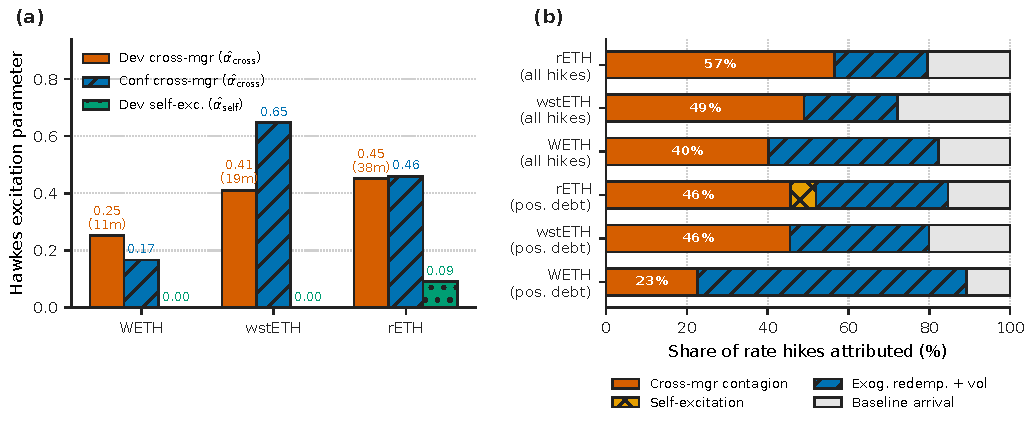
\includegraphics[width=0.98\textwidth]{figures/fig4_hawkes_leapfrogging.pdf}
\caption{Multivariate Hawkes cross-manager leapfrogging estimates and hike-intensity attribution. Panel~(a) contrasts positive-debt cross-manager excitation $\hat{\alpha}_{\text{cross}}$ across Development (with cross-excitation half-life in minutes) and Confirmation against same-manager self-excitation $\hat{\alpha}_{\text{self}}$. Panel~(b) decomposes observed rate hikes into baseline arrival, exogenous redemption and volatility shocks, self-excitation, and cross-manager contagion across all genuine hikes and positive-debt hikes in the pooled 485-day sample.}
\label{fig:hawkes}
\end{figure}

An institutional contract constraint explains why $\hat{\alpha}_{\text{self}} = 0.000$ on WETH and wstETH. Because \texttt{MIN\_INTEREST\_RATE\_CHANGE\_PERIOD} $= 3{,}600$~seconds strictly enforces zero same-manager gaps below one hour, same-manager self-excitation is mechanically blocked across the 11-to-19-minute cross-manager decay window. Post-1-hour gap diagnostics confirm this mechanism: only 3 of 98 (3.06\%) same-manager hike gaps on WETH and 6 of 266 (2.26\%) on wstETH fall inside $[1\text{h}, 2\text{h})$, whereas rETH exhibits 19 of 145 (13.10\%) same-manager gaps in $[1\text{h}, 2\text{h})$ alongside a 37.61-minute decay half-life and a correspondingly positive $\hat{\alpha}_{\text{self}} = 0.091$ in Development (0.064 Pooled). Rival managers face no mutual 1-hour lock against one another, so Edgeworth leapfrogging cascades unimpeded across competing batches within minutes.

\section{Structural estimation, equilibrium welfare, and cross-protocol benchmark}\label{sec:structural}

\subsection{Complete transaction-level gas accounting}\label{subsec:gas}

Gas savings cannot bridge the repricing gap. A natural defense of delegated borrowing is that pooling dozens of troves inside one batch amortizes Ethereum execution gas across borrowers. To test whether gas economies offset the $+38.04$~BOLD per million debt-days liability disadvantage documented in Table~\ref{tab:sample_overview}, we match exact transaction-level gas fees (converted at daily ETH/USD prices) across the entire 485-day ledger.

Matching achieves 100.00\% coverage on all user and batch-manager transactions (11,421 of 11,421 transactions; 11,423 of 11,444 overall, with all 21 unmatched Development hashes verified as initial protocol deployment and administrative setup calls). Total execution gas across 485~days equals 10.7107~ETH, or \usd31,566.77 (\usd29,425.11 Development across 9,677 user transactions and \usd2,141.66 Confirmation across 1,744 user transactions). Allocating the 334 mixed-group transactions proportionally by event exposure yields pooled delegated gas of 1.074~BOLD per million debt-days (extreme all-to-delegated and zero-to-delegated allocation bounds $[1.007, 1.202]$) versus 2.149~BOLD per million debt-days for unbatched debt (bounds $[2.072, 2.189]$). The resulting delegated gas advantage of $-1.074$~BOLD per million debt-days (3.92~bp/yr versus 7.84~bp/yr; $-0.944$ in Development and $-1.320$ in Confirmation) is 35~times too small to offset the $+38.04$~BOLD per million debt-days upfront-fee penalty. Batch rate updates themselves cost only \usd1,866.42 in total gas across 485~days (\usd572.20 on staircase hikes). Managers thus pay pennies in execution gas while capitalizing hundreds of thousands of dollars in cooldown penalties onto borrower principal.

\subsection{Within-day nonparametric cost inversion and out-of-sample validation}\label{subsec:gpv}

Moving from accounting liabilities to structural welfare requires recovering borrowers' latent per-dollar redemption-disruption costs $\tau_i$ directly from equilibrium rate choices. Following \citet{guerre2000optimal} and our reverse-priority-queue inversion identity \eqref{eq:gpv_inv}, we first map 5,005 of 5,026 (99.58\%) canonical on-chain trove redemption hits onto their exact pre-redemption normalized queue quantile $s = q/D \in [0, 1]$ and estimate the empirical depth-dependent hazard curve $\hat{\lambda}(s)$ via a Pareto-power specification (pooled bin-fit $R^2 = 0.9964$; WETH $0.9784$, wstETH $0.9930$, rETH $0.9097$). Realized redemption intensity plunges sharply down the queue: pooled empirical hazard drops from 12.90/yr in the first 5\% queue vingtile ($[0\%, 5\%]$) to 2.59/yr in the second ($[5\%, 10\%]$), 0.69/yr in the third ($[10\%, 15\%]$), and 0.04/yr in the fifth and sixth vingtiles ($[20\%, 30\%]$).

Naive time pooling severely distorts structural cost estimates. Because macro interest rates drifted across our 485-day window, pooling all daily snapshots into a single unconditional rate CDF mixes time-series rate shifts with cross-sectional queue dispersion, inflating the apparent quantile slope $(F^{-1})'(s)$ and biasing recovered disruption costs upward by 3.18~times at the median (1,151.9~bp pooled versus 362.0~bp within-day) and 5.53~times at the 25th percentile (523.4~bp versus 94.6~bp). To match our theoretical daily queue equilibrium cleanly, we compute the debt-weighted average within-(branch, day) cross-sectional quantile curve $\bar{Q}(s)$ across all 1,455 branch-day cells (1,224 in Development), estimate $\bar{Q}'(s)$ via Gaussian-weighted local-linear regression ($h = 0.06$), invert \eqref{eq:gpv_inv} at the empirical median realized redemption fee $\hat{\phi} = 0.721\%$, and apply Pool-Adjacent-Violators (PAVA) isotonic projection to the raw inverted schedule $\hat{\tau}_{\text{raw}}(s)$.

\begin{table}[!htbp]
\centering
\caption{Within-day nonparametric GPV cost inversion, out-of-sample validation, and general-equilibrium welfare counterfactuals.}
\label{tab:gpv_welfare}
\footnotesize
\setlength{\tabcolsep}{3.8pt}
\resizebox{\textwidth}{!}{\begin{tabular}{@{}lrrrrrrrr@{}}
\toprule
\multicolumn{9}{@{}l}{\textit{Panel A: Within-(branch, day) debt-weighted GPV structural estimates and welfare decomposition (Pooled, 485d)}} \\
\midrule
Branch & $p_0$ (\%) & Med.\ $\hat{\tau}$ (bp) & IQR $\hat{\tau}$ (bp) & GOF RMSE & $C_{\text{PQ}}$ & $T_{\text{PQ}}$ sprd/tot & $\text{PoA}_{\text{sprd}}$ / $\text{PoA}_{\text{tot}}$ & OOS RMSE \\
\midrule
All branches (1,455 cells) & 3.87 & 362.0 & $[94.6, 1{,}984]$ & 2.8~bp & 74.2 & 52.8 / 301.4 & $1.713\times$ / $5.065\times$ & 42.2~bp \\
\quad Development (1,224 cells) & 4.28 & 326.8 & $[92.8, 1{,}912]$ & 2.4~bp & 74.7 & 49.0 / 295.5 & $1.656\times$ / $4.955\times$ & -- \\
WETH (485 cells) & 0.78 & 977.8 & $[109.2, 5{,}176]$ & 11.6~bp & 125.5 & 100.4 / 303.3 & $1.800\times$ / $3.417\times$ & 90.8~bp \\
wstETH (485 cells) & 4.84 & 237.6 & $[94.0, 1{,}472]$ & 2.5~bp & 56.0 & 40.7 / 300.6 & $1.727\times$ / $6.370\times$ & 10.8~bp \\
rETH (485 cells) & 5.72 & 75.9 & $[75.9, 276]$ & 9.7~bp & 37.2 & 13.8 / 301.6 & $1.372\times$ / $9.113\times$ & 343.9~bp \\
\midrule
\multicolumn{9}{@{}l}{\textit{Panel B: General-equilibrium best-response welfare counterfactuals (Pooled 485d, baseline $\varepsilon_{\text{SP}} = 0.50$)}} \\
\midrule
Counterfactual regime & $m^*$ & Eq.\ $r^*$ & Borr.\ upf & Obs.\ fin.\ & $C_{\text{PQ}}$ & All-in welf.\ & $\Delta$ welf.\ / $\Delta$ DWL & Eq.\ SP APR \\
 & (mult.) & (bp) & (bp) & (bp) & (bp) & (bp) & (bp vs.\ SQ) & (\%) \\
\midrule
Status Quo & 1.0000 & 318.0 & 226.2 & 576.0 & 74.2 & 653.5 & $+0.0$ / $+0.0$ & 4.97\% \\
Baseline $\DesignA$ (with leak) & 1.0685 & 328.5 & 29.7 & 390.1 & 79.2 & 469.4 & $-184.1$ / $+1.9$ & 4.35\% \\
$\DesignAStar$ (0-slot optimal) & 1.0623 & 334.7 & 39.0 & 405.6 & 78.8 & 484.4 & $-169.1$ / $+1.5$ & 4.40\% \\
$\DesignD$ (1-slot escrow) & 1.0707 & 337.0 & 15.6 & 384.5 & 79.4 & 463.9 & $-189.5$ / $+2.1$ & 4.34\% \\
Co-Pay $\beta = 0.10$ (on SQ) & 1.0112 & 321.0 & 171.6 & 524.2 & 75.0 & 601.1 & $-52.4$ / $-0.7$ & 4.86\% \\
Co-Pay $\beta = 0.25$ (on SQ)* & 1.0218 & 323.9 & 130.1 & 485.4 & 75.8 & 562.3 & $-91.2$ / $-0.9$ & 4.76\% \\
Co-Pay $\beta = 0.50$ (on SQ)* & 1.0324 & 326.7 & 98.0 & 456.0 & 76.5 & 533.2 & $-120.3$ / $-0.7$ & 4.66\% \\
$\DesignAStar$ + Co-Pay $\beta = 0.25$ & 1.0667 & 335.9 & 20.1 & 387.5 & 79.1 & 466.6 & $-186.9$ / $+1.4$ & 4.37\% \\
\midrule
\multicolumn{9}{@{}l}{\textit{Panel C: Parametric Stability Pool elasticity grid for $\DesignAStar$ (Pooled 485d, unique fixed point at each $\varepsilon_{\text{SP}}$)}} \\
\midrule
SP supply elasticity $\varepsilon_{\text{SP}}$ & $m^*$ & Eq.\ $r^*$ & Borr.\ upf & Obs.\ fin.\ & $\Delta$ fin.\ & All-in welf.\ & $\Delta$ DWL & Eq.\ SP APR \\
\midrule
$\varepsilon_{\text{SP}} = 0.00$ (static) & 1.0000 & 318.0 & 36.7 & 386.5 & $-189.5$ & 460.7 & $-3.2$ & 4.18\% \\
$\varepsilon_{\text{SP}} = 0.25$ (low GE) & 1.0363 & 327.8 & 38.0 & 397.6 & $-178.4$ & 474.5 & $-0.5$ & 4.31\% \\
$\varepsilon_{\text{SP}} = 0.50$ (baseline GE) & 1.0623 & 334.7 & 39.0 & 405.6 & $-170.5$ & 484.4 & $+1.5$ & 4.40\% \\
$\varepsilon_{\text{SP}} = 1.00$ (elastic GE) & 1.0971 & 344.1 & 40.2 & 416.2 & $-159.8$ & 497.6 & $+4.1$ & 4.53\% \\
$\varepsilon_{\text{SP}} = 2.00$ (high GE) & 1.1346 & 354.1 & 41.6 & 427.6 & $-148.4$ & 511.9 & $+6.9$ & 4.67\% \\
\bottomrule
\end{tabular}}
\par\vspace{4pt}\begin{minipage}{\textwidth}\footnotesize\setlength{\parskip}{0pt}\textit{Notes.} Panel A inverts \eqref{eq:gpv_inv} on debt-weighted average within-(branch, day) quantile curves across all 485~days ($p_0$ is the absorber share at $r_{\min}$; GOF RMSE measures in-sample fit over $[p_0, 0.92]$; OOS RMSE evaluates Development-estimated cost distributions predicting Confirmation queue spreads above Confirmation's empirical front rate $r_{\text{front,conf}}$). $T_{\text{PQ}}$ and borrower PoA are reported under both spread above empirical floor $r_{\text{front}}$ ($293.9$~bp all-branch) and total interest above $r_{\min} = 50$~bp. Panels B and C solve the macro SP-yield fixed point with zero ad hoc mis-sorting floor ($\text{mis\_sort} = 0.0$~bp), conservative $1.00\times$ update frequency for $\DesignA/\DesignAStar/\DesignD$, cubic-root HJB frequency scaling for Co-Pay ($\alpha_{\text{SQ}} = 0.2472$), observed March 6, 2026 leakage ($7.85$~bp/yr) for baseline $\DesignA$, and full $m^* C_{\text{PQ}}$ in social DWL; all $\Delta$ columns report $\text{counterfactual} - \text{SQ}$ in bp/yr (negative denotes lower borrower cost or lower social DWL; positive denotes higher social DWL). Asterisked standalone Co-Pay rows ($\beta \ge 0.25$ on SQ) fail self-funding feasibility against the 27.9~bp management fee, whereas $\DesignAStar + \text{Co-Pay }\beta=0.25$ is fully self-funding.
\end{minipage}
\end{table}

Panel A of Table~\ref{tab:gpv_welfare} and Figure~\ref{fig:gpv}(a) report the structural inversion results. Across all branches pooled, the absorber fraction at $r_{\min}$ equals $p_0 = 3.87\%$ (4.28\% Development), 100.0\% of quantiles satisfy strict GPV rationalizability (Spearman $\rho = 1.000$; WETH and wstETH likewise achieve 100.0\% with $\rho = 1.000$, while thin rETH reaches 70.3\% pre-PAVA monotonicity with $\rho = 0.533$), and the recovered median gross borrower disruption cost is 362.0~bp (3.62\% per dollar redeemed; IQR $[94.6, 1{,}983.5]$~bp; 14-day block-bootstrap 95\% CI $[264.7, 526.5]$~bp; bandwidth sensitivity 333.2~bp at $0.75h$ and 404.2~bp at $1.50h$). That 3.62\% median cost lines up closely with real-world DeFi borrower frictions: DEX slippage, re-borrowing origination fees, and taxable realization of unrealized ETH capital gains. Re-integrating the inverted cost distribution through \eqref{eq:rpq_eq} reproduces the empirical cross-sectional rate curve with an in-sample quantile RMSE of just 2.8~bp (2.4~bp in Development; 2.5~bp on wstETH). Cross-branch heterogeneity aligns with collateral composition: WETH troves display the highest median disruption cost (977.8~bp, $p_0 = 0.78\%$), wstETH sits near the middle (237.6~bp, $p_0 = 4.84\%$), and thin rETH carries the lowest median cost (75.9~bp, $p_0 = 5.72\%$).

Structural welfare decomposition confirms the large sorting efficiency of the reverse priority queue alongside substantial positional rent transfer. Across all branches pooled, equilibrium priority-queue redemption disruption equals $C_{\text{PQ}} = 74.2$~bp/yr (56.8~bp/yr truncated at the 90th quantile), substantially lower than random pro-rata redemption ($3{,}952.5$~bp/yr full support; $2{,}865.0$~bp/yr truncated at 90\%), which yields a large sorting gain. Measuring borrower positional interest transfers above the empirical front-of-queue rate floor ($r_{\text{front}} = 293.9$~bp) yields $T_{\text{PQ,spread}} = 52.8$~bp/yr, $E_{\text{PQ}} - r_{\text{front}} = 127.0$~bp/yr, and a borrower Price of Anarchy of $\text{PoA}_{\text{spread}} = 1.713\times$. Measuring total interest above the statutory protocol floor $r_{\min} = 50.0$~bp yields $T_{\text{PQ,total}} = 301.4$~bp/yr, $E_{\text{PQ,total}} = 375.6$~bp/yr, and $\text{PoA}_{\text{total}} = 5.065\times$. Both ratios lie orders of magnitude below the homogeneous-type all-pay rent-dissipation benchmark ($184.3\times$); borrower type heterogeneity thus preserves meaningful allocative efficiency.

Out-of-sample validation from Development to frozen Confirmation tests the structural model against a genuine macro regime shift. Holding the Development-estimated cost distribution $\hat{H}_{\text{Dev}}$ fixed and feeding Confirmation's realized redemption intensity into \eqref{eq:rpq_eq} above Confirmation's empirical queue floor $r_{\text{front,conf}}$, the model fits wstETH tightly (observed spread 66.5~bp versus predicted 56.2~bp; mean error $-10.3$~bp, quantile RMSE 10.8~bp). On WETH ($r_{\text{front,conf}} = 155.6$~bp), a small mean spread error (131.9~bp observed versus 133.8~bp predicted, $+1.9$~bp) masks cross-quantile curvature cancellation (quantile RMSE 90.8~bp), while across all branches ($r_{\text{front,conf}} = 283.7$~bp), observed spread reaches 107.0~bp against 64.9~bp predicted (mean error $-42.1$~bp, RMSE 42.2~bp), and thin rETH shifts sharply (353.1~bp versus 9.3~bp, RMSE 343.9~bp). The economic reason for this divergence is transparent in the data: realized redemption turnover plunged 3.72-fold between Development and the 77-day Confirmation window (from 2.771/yr to 0.745/yr), yet posted Confirmation rates rose $+45.2$~bp. Borrowers priced forward-looking tail-risk redemption expectations inside the calm 77-day holdout even when few redemptions materialized, a classic peso-problem wedge between realized short-horizon turnover and ex ante queue risk.

\subsection{General-equilibrium best-response welfare counterfactuals}\label{subsec:ge_welfare}

Evaluating protocol fee reforms solely on fixed historical actions ignores equilibrium feedback: cutting borrower upfront fees reduces Stability Pool APR (since 75\% of upfront fees flow to SP depositors), which may induce SP outflows, raise unbacked debt and redemption arrival intensity by an equilibrium multiplier $m^* \ge 1$, push equilibrium base rates $r^*$ upward along \eqref{eq:rpq_eq}, and lift total redemption disruption to $m^* C_{\text{PQ}}$. We solve this full two-sided general-equilibrium fixed point cleanly under four strict discipline rules. First, we strip out any ad hoc queue mis-sorting bonus ($\text{mis\_sort} = 0.0$~bp; raw within-day rate-staleness correlation is $-0.0031$). Second, we hold update frequency conservatively at $1.00\times$ under $\DesignA$, $\DesignAStar$, and $\DesignD$ while deriving Co-Pay frequency attenuation strictly from our cubic-root HJB elasticity $(\alpha_{\text{SQ}} / \alpha_{\text{eff}}(\beta))^{2/3}$ calibrated to $\alpha_0 = 0.25$ ($\alpha_{\text{SQ}} = 0.2472$). Third, we calibrate baseline $\DesignA$'s spike-and-cut leakage directly to the observed March 6, 2026 mainnet exploits ($7.85$~bp/yr pooled). Fourth, we include the full equilibrium redemption disruption $m^* C_{\text{PQ}}$ inside net social deadweight loss so zero phantom welfare gains appear. Because weekly empirical SP-yield elasticity regressions are statistically underpowered ($N = 60$ weeks, slope $-0.39$, $\text{SE} = 0.454$, $p = 0.394$; Development $p = 0.922$), we report our baseline at $\varepsilon_{\text{SP}} = 0.50$ alongside the complete 5-point parametric grid $\varepsilon_{\text{SP}} \in \{0.00, 0.25, 0.50, 1.00, 2.00\}$.

\begin{figure}[!htbp]
\centering
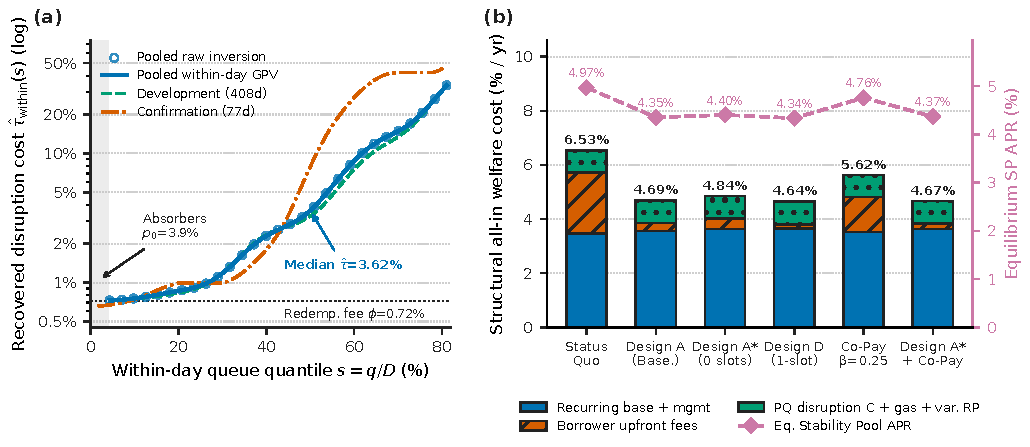
\includegraphics[width=0.98\textwidth]{figures/fig5_gpv_structural_welfare.pdf}
\caption{Within-day nonparametric GPV disruption-cost curve and general-equilibrium welfare counterfactuals. Panel~(a) plots the recovered within-(branch, day) gross borrower disruption cost $\hat{\tau}_{\text{within}}(s)$ (log scale) against normalized queue quantile $s = q/D$ across Pooled, Development, and Confirmation samples, marking the 3.87\% absorber pool and 362.0~bp median cost. Panel~(b) stacks equilibrium borrower welfare components (recurring base plus management APR, borrower upfront fees, and queue disruption plus gas and episodic variance risk premium) on the left axis against equilibrium Stability Pool APR (right axis) across regimes at baseline $\varepsilon_{\text{SP}} = 0.50$.}
\label{fig:gpv}
\end{figure}

Panels B and C of Table~\ref{tab:gpv_welfare} and Figure~\ref{fig:gpv}(b) present the equilibrium welfare outcomes. Under Status Quo at baseline $\varepsilon_{\text{SP}} = 0.50$, delegated borrowers face 576.0~bp/yr in observed financial cost (318.0~bp base APR + 27.9~bp management fee + 226.2~bp upfront repricing fees + 3.9~bp gas) and 653.5~bp/yr in structural all-in welfare cost (adding 74.2~bp disruption $C_{\text{PQ}}$ and 3.3~bp episodic variance risk premium), and protocol revenue supports a 4.97\% Stability Pool APR (scaling the Section~\ref{subsec:theory} yield identity by the empirical SP-to-debt coverage ratio $\text{SP}/D = 0.6753$, so $y_{\text{SP}} = \eta \bar{R}_{\text{eff}} / (\text{SP}/D) = 0.75 \times 4.476\% / 0.6753 = 4.97\%$ under Status Quo). Switching to zero-storage $\DesignAStar$ drives a unique fixed point at $m^* = 1.0623$: equilibrium base APR rises modestly by $+16.7$~bp (from 318.0 to 334.7~bp) and SP APR settles at 4.40\% ($-57$~bp), while borrower upfront fees drop by 187.2~bp (226.2 to 39.0~bp). Net borrower observed financial cost falls by $-170.5$~bp (576.0 to 405.6~bp) and structural all-in welfare cost falls by $-169.1$~bp (653.5 to 484.4~bp). Hardened one-slot $\DesignD$ delivers an even larger $-191.5$~bp financial reduction (to 384.5~bp, or 3.85\%, with all-in welfare $-189.5$~bp at $m^* = 1.0707$ and SP APR 4.34\%).

The two-sided decomposition reveals an essential economic truth about yield-recycling stablecoins. Almost the entire 170.5~bp borrower gain under $\DesignAStar$ is an avoided involuntary pecuniary transfer to SP and PIL recipients ($-170.5$~bp transfer change), whereas net pure social deadweight loss increases by only $+1.5$~bp at $\varepsilon_{\text{SP}} = 0.50$ (from 81.4 to 82.8~bp, spanning a $-3.2$~bp reduction at $\varepsilon_{\text{SP}} = 0.00$ where episodic variance risk drops without higher redemption turnover up to a $+6.9$~bp increase at high elasticity $\varepsilon_{\text{SP}} = 2.00$, where $m^* = 1.1346$ lifts equilibrium redemption disruption from 74.2 to 84.1~bp). Even at extreme $\varepsilon_{\text{SP}} = 2.00$, borrowers still save $-148.4$~bp in financial cost (427.6~bp versus 576.0~bp) while SP APR holds at 4.67\%. For governance, Panel B also verifies the co-pay feasibility trade-off predicted in Section~\ref{subsec:theory}: imposing a standalone 25\% or 50\% manager co-pay on top of Status Quo is insolvent against the 27.9~bp annual management fee (leaving managers with negative net cash flow), whereas pairing $\DesignAStar$ with a 25\% co-pay is strictly self-funding (managers pay just 6.7~bp out of 27.9~bp revenue), cuts borrower financial cost to 387.5~bp ($-188.6$~bp versus SQ), and eliminates zero-redemption near-notch churning.

\subsection{Apples-to-apples cross-protocol borrowing cost benchmark}\label{subsec:cross_protocol}

Cooldown friction alone flips BOLD's competitive position in decentralized credit markets. Table~\ref{tab:cross_protocol} and Figure~\ref{fig:benchmark}(a) compare Liquity V2's exact 485-day observed and general-equilibrium financial borrowing costs against every major live overcollateralized Ethereum stablecoin and variable money-market benchmark over the identical May 19, 2025--September 15, 2026 window: Liquity V1 (LUSD), Sky/MakerDAO (DAI/USDS \texttt{ETH-A} and \texttt{WSTETH-A}), Curve (\texttt{crvUSD} WETH and wstETH), and Aave V3 (\texttt{GHO} and \texttt{USDC} variable borrow).

To enforce apples-to-apples scope transparency, Table~\ref{tab:cross_protocol} reports ongoing repricing-only upfront fees as the primary benchmark (\texttt{BatchUpdated} for delegated BOLD versus \texttt{op=3} for unbatched BOLD) and explicitly states the all-upfront scope including initial origination, draw, and batch-join charges ($+0.253\%$/yr delegated versus $+0.320\%$/yr unbatched) in the table notes and text. Counterfactual BOLD rows display Status Quo peg RMSE ($22.93^*$~bp) and rate standard deviation ($1.18\%$) strictly as ceteris paribus reference values, while non-BOLD rows conservatively omit wallet execution gas (approximately 4--8~bp/yr).

\begin{table}[!htbp]
\centering
\caption{Apples-to-apples cross-protocol financial borrowing cost, rate volatility, and peg stability benchmark (485~days).}
\label{tab:cross_protocol}
\footnotesize
\setlength{\tabcolsep}{4.5pt}
\resizebox{\textwidth}{!}{\begin{tabular}{@{}lrrrrrr@{}}
\toprule
Protocol and collateral scope & Quoted & Episodic / & Obs.\ financial & Rate SD & Peg RMSE & Min USD \\
(Repricing-only scope for BOLD) & APR (\%) & upfront (\%) & cost (\%) & (\%) & (bp) & price \\
\midrule
Liquity V2 (BOLD): Delegated (Status Quo) & 3.46 & 2.262 & 5.76 & 1.18 & 22.93 & \usd0.99247 \\
Liquity V2 (BOLD): Unbatched (Self-Managed) & 3.72 & 0.176 & 3.97 & 0.94 & 22.93 & \usd0.99247 \\
Liquity V2 (BOLD): Delegated ($\DesignAStar$ GE) & 3.63 & 0.390 & 4.06 & 1.18 & 22.93* & \usd0.99247 \\
Liquity V2 (BOLD): Delegated ($\DesignD$ GE) & 3.65 & 0.157 & 3.85 & 1.18 & 22.93* & \usd0.99247 \\
\addlinespace[4pt]
Liquity V1 (LUSD, 1-year horizon) & 0.00 & 0.526 & 0.53 & 0.08 & 59.33 & \usd0.99307 \\
Sky / MakerDAO (DAI/USDS: ETH-A) & 7.88 & 0.000 & 7.88 & 0.93 & 4.10 & \usd0.99533 \\
Sky / MakerDAO (DAI/USDS: WSTETH-A) & 8.88 & 0.000 & 8.88 & 0.93 & 4.27 & \usd0.99818 \\
Curve (crvUSD: WETH) & 5.68 & n/a & 5.68 & 4.72 & 15.25 & \usd0.98642 \\
Curve (crvUSD: wstETH) & 6.36 & n/a & 6.36 & 4.71 & 15.25 & \usd0.98642 \\
Aave V3 (GHO, base prior to rebates) & 4.54 & 0.000 & 4.54 & 0.96 & 9.78 & \usd0.99767 \\
Aave V3 (USDC Variable Borrow) & 5.30 & 0.000 & 5.30 & 2.20 & n/a & n/a \\
\bottomrule
\end{tabular}}
\par\vspace{4pt}\begin{minipage}{\textwidth}\footnotesize\setlength{\parskip}{0pt}\textit{Notes.} Sample spans May 19, 2025--September 15, 2026 (485~days; 477~days for BOLD prices from May 27, 2025). All Liquity V2 rows use exact debt-day weighted APRs (base plus management fee for delegated: 3.18\% + 0.28\% = 3.46\% SQ; 3.35\% + 0.28\% = 3.63\% $\DesignAStar$ GE; 3.37\% + 0.28\% = 3.65\% $\DesignD$ GE) plus Replay-computed repricing fees and allocated gas (0.04\% delegated, 0.08\% unbatched). Including origination, draw, and batch-join fees ($+0.253\%$ delegated, $+0.320\%$ unbatched) yields all-upfront financial costs of 6.01\% Delegated SQ, 4.29\% Unbatched, 4.31\% $\DesignAStar$ GE, and 4.10\% $\DesignD$ GE. Asterisked counterfactual BOLD peg RMSEs ($22.93^*$~bp) and rate SDs are Status Quo ceteris paribus reference values. Liquity V1 reflects a one-time minting fee annualized at a 1-year horizon (2.10\%/yr at 3~months; 0.26\%/yr at 2~years). Curve \texttt{crvUSD} excludes unobserved path-dependent LLAMMA soft-liquidation losses; Sky rates are exact compounded APY from 71/71 weekly archive blocks (\texttt{Jug.base} $= 0$); Aave V3 rates are nominal APR from 71/71 weekly archive blocks (GHO prior to \texttt{stkAAVE}/Merit discounts); non-BOLD rows omit wallet gas.
\end{minipage}
\end{table}

The cross-protocol comparison clarifies the market-structure stakes. Quoted rates invert the true cost ranking. Judged solely on quoted APR (3.46\%), delegated Liquity V2 appears 108~bp cheaper than Aave V3 GHO (4.54\%), 184~bp cheaper than Aave V3 USDC (5.30\%), 222~bp cheaper than Curve crvUSD WETH (5.68\%), and 442~bp cheaper than Sky ETH-A (7.88\%). Once actual Status Quo repricing penalties (2.262\%) and gas (0.039\%) enter the ledger, delegated BOLD's observed financial cost jumps to 5.76\% (6.01\% all-upfront), becoming 122~bp more expensive than Aave GHO, 46~bp more expensive than Aave USDC, and 8~bp more expensive than Curve crvUSD WETH, while trailing only Sky's governance-set 7.88\%--8.88\% vaults. Unbatched self-managed BOLD tells a different story. At 3.97\% financial cost (4.29\% all-upfront), self-managed BOLD beats every variable-rate peer except zero-interest Liquity V1 LUSD, whose peg stability is 2.6~times looser (59.33~bp RMSE versus BOLD's 22.93~bp).

\begin{figure}[!htbp]
\centering
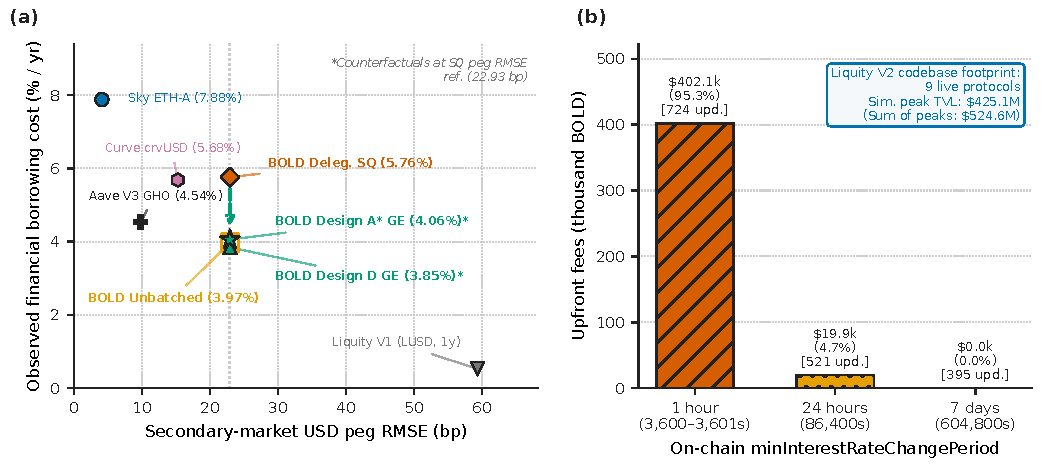
\includegraphics[width=0.98\textwidth]{figures/fig6_cross_protocol_benchmark.pdf}
\caption{Cross-protocol borrowing-cost versus peg-stability frontier and Liquity V2 permission footprint. Panel~(a) plots 485-day observed financial borrowing cost against secondary-market USD peg RMSE across Liquity V2 (Status Quo, Unbatched, $\DesignAStar$ GE, and $\DesignD$ GE), Liquity V1 LUSD, Aave V3 GHO, Curve crvUSD, and Sky ETH-A. Panel~(b) summarizes total 485-day borrower upfront fees across immutable manager \texttt{minInterestRateChangePeriod} floors alongside the verified nine-protocol Liquity V2 friendly-fork TVL footprint (\usd425.1M simultaneous peak; \usd524.6M sum of peaks).}
\label{fig:benchmark}
\end{figure}

Adopting either $\DesignAStar$ or $\DesignD$ reverses that competitive penalty in general equilibrium. At $\varepsilon_{\text{SP}} = 0.50$, $\DesignAStar$ lowers delegated BOLD's financial cost to 4.06\% (4.31\% all-upfront) and $\DesignD$ lowers it to 3.85\% (4.10\% all-upfront), moving delegated BOLD decisively back below Aave GHO (4.54\%), Aave USDC (5.30\%), Curve crvUSD WETH (5.68\%) and wstETH (6.36\%), and Sky (7.88\%--8.88\%), while avoiding crvUSD's 4.72\% rate volatility and unobserved LLAMMA rebalancing losses and maintaining a 2.6-fold peg-RMSE advantage over Liquity V1. Figure~\ref{fig:benchmark}(b) documents the industry-wide reach of this architectural fix: because 95.3\% of all Status Quo borrower penalties originate from 1-hour-floor managers operating under the exact same cooldown contract copied across nine live Liquity V2 deployments peaking simultaneously at \usd425.06~million TVL, replacing fixed branch-average cooldown fees with symmetric incremental charges or one-slot rate-bond escrow improves delegated borrowing across the entire user-set-rate stablecoin class.

\section{Concluding remarks}\label{sec:conclusion}

Delegated interest-rate management solves borrower attention costs inside user-set-rate stablecoins, yet interacts destructively with fixed branch-average cooldown penalties. Across 485~days of canonical Ethereum mainnet activity for Liquity V2, delegated loans advertise 40.15 to 55.44~bp lower base APRs while inflicting 38.04~BOLD per million debt-days higher total financing liabilities (5.76\% versus 3.97\% annualized financial cost). Live on-chain permission tuples, 168-hour notch bunching ($b = 91.8$, $+57.8$~pp hike-versus-cut asymmetry), dominated near-notch hikes costing up to 9,207~BOLD hours before free expiry, live March 6, 2026 spike-and-cut arbitrage extracting 84.02\% and 60.96\% discounts, mechanical-routing Bartik 2SLS (+13.53~BOLD per million debt-days), and multivariate Hawkes leapfrogging ($\hat{\alpha}_{\text{cross}} \in [0.17, 0.65]$) all converge on a single economic mechanism: contractual incidence separates who pays the lumpy penalty from who presses the rate-update button.

These results carry direct design lessons for decentralized financial intermediation. First, borrower-side delegation exhibits a mirror-image agency friction to lender-side vault curation \citep{chitra2025curationary,mancino2026sok}: whereas lender curators risk reaching for yield at depositor liquidation expense, liability managers risk over-reacting to redemption salience at borrower principal-capitalization expense. Second, protocol-level fee structure dominates client-side keeper heuristics. Replacing fixed branch-average cooldown charges with zero-storage symmetric incremental fees ($\DesignAStar$) or hardened one-slot principal-escrow ($\DesignD$) preserves anti-front-running security across all four contract rate-transition paths, eliminates live spike-and-cut arbitrage completely, cuts delegated repricing fees by 83.8\% to 93.5\%, enables self-funded manager co-pays, and restores delegated BOLD (3.85\%--4.06\%) as the lowest-cost variable-rate decentralized stablecoin across Ethereum peers without sacrificing peg discipline.

Three explicit scope boundaries qualify our empirical findings. First, Ethereum collateral markets operated inside a relatively calm liquidation regime during our 485-day window (63 liquidations in Development and zero in Confirmation), so extreme correlated collateral crashes remain outside sample support. Second, although our nine-deployment codebase footprint reached \usd425.06~million in simultaneous peak TVL, canonical Ethereum BOLD debt averaged 37.3~million~BOLD over the sample, and weekly Stability Pool supply-elasticity estimates are statistically imprecise ($p = 0.394$), which is why we present general-equilibrium welfare across the full five-point elasticity grid $\varepsilon_{\text{SP}} \in [0.00, 2.00]$. Third, all counterfactual mechanisms are evaluated pre-deployment via exact state replay and structural equilibrium inversion; formal machine-checked Lean~4 security proofs, compiled Solidity storage-layout diffs, and runtime EVM gas benchmarks are established in \citet{companion2026}. Taken together, the evidence shows that immutable smart contracts solve issuer time-inconsistency only when their fee rules align delegated agents' marginal update incentives with the borrowers who fund the protocol.
